% Options for packages loaded elsewhere
\PassOptionsToPackage{unicode}{hyperref}
\PassOptionsToPackage{hyphens}{url}
%
\documentclass[
]{book}
\usepackage{amsmath,amssymb}
\usepackage{iftex}
\ifPDFTeX
  \usepackage[T1]{fontenc}
  \usepackage[utf8]{inputenc}
  \usepackage{textcomp} % provide euro and other symbols
\else % if luatex or xetex
  \usepackage{unicode-math} % this also loads fontspec
  \defaultfontfeatures{Scale=MatchLowercase}
  \defaultfontfeatures[\rmfamily]{Ligatures=TeX,Scale=1}
\fi
\usepackage{lmodern}
\ifPDFTeX\else
  % xetex/luatex font selection
\fi
% Use upquote if available, for straight quotes in verbatim environments
\IfFileExists{upquote.sty}{\usepackage{upquote}}{}
\IfFileExists{microtype.sty}{% use microtype if available
  \usepackage[]{microtype}
  \UseMicrotypeSet[protrusion]{basicmath} % disable protrusion for tt fonts
}{}
\makeatletter
\@ifundefined{KOMAClassName}{% if non-KOMA class
  \IfFileExists{parskip.sty}{%
    \usepackage{parskip}
  }{% else
    \setlength{\parindent}{0pt}
    \setlength{\parskip}{6pt plus 2pt minus 1pt}}
}{% if KOMA class
  \KOMAoptions{parskip=half}}
\makeatother
\usepackage{xcolor}
\usepackage{color}
\usepackage{fancyvrb}
\newcommand{\VerbBar}{|}
\newcommand{\VERB}{\Verb[commandchars=\\\{\}]}
\DefineVerbatimEnvironment{Highlighting}{Verbatim}{commandchars=\\\{\}}
% Add ',fontsize=\small' for more characters per line
\usepackage{framed}
\definecolor{shadecolor}{RGB}{248,248,248}
\newenvironment{Shaded}{\begin{snugshade}}{\end{snugshade}}
\newcommand{\AlertTok}[1]{\textcolor[rgb]{0.94,0.16,0.16}{#1}}
\newcommand{\AnnotationTok}[1]{\textcolor[rgb]{0.56,0.35,0.01}{\textbf{\textit{#1}}}}
\newcommand{\AttributeTok}[1]{\textcolor[rgb]{0.13,0.29,0.53}{#1}}
\newcommand{\BaseNTok}[1]{\textcolor[rgb]{0.00,0.00,0.81}{#1}}
\newcommand{\BuiltInTok}[1]{#1}
\newcommand{\CharTok}[1]{\textcolor[rgb]{0.31,0.60,0.02}{#1}}
\newcommand{\CommentTok}[1]{\textcolor[rgb]{0.56,0.35,0.01}{\textit{#1}}}
\newcommand{\CommentVarTok}[1]{\textcolor[rgb]{0.56,0.35,0.01}{\textbf{\textit{#1}}}}
\newcommand{\ConstantTok}[1]{\textcolor[rgb]{0.56,0.35,0.01}{#1}}
\newcommand{\ControlFlowTok}[1]{\textcolor[rgb]{0.13,0.29,0.53}{\textbf{#1}}}
\newcommand{\DataTypeTok}[1]{\textcolor[rgb]{0.13,0.29,0.53}{#1}}
\newcommand{\DecValTok}[1]{\textcolor[rgb]{0.00,0.00,0.81}{#1}}
\newcommand{\DocumentationTok}[1]{\textcolor[rgb]{0.56,0.35,0.01}{\textbf{\textit{#1}}}}
\newcommand{\ErrorTok}[1]{\textcolor[rgb]{0.64,0.00,0.00}{\textbf{#1}}}
\newcommand{\ExtensionTok}[1]{#1}
\newcommand{\FloatTok}[1]{\textcolor[rgb]{0.00,0.00,0.81}{#1}}
\newcommand{\FunctionTok}[1]{\textcolor[rgb]{0.13,0.29,0.53}{\textbf{#1}}}
\newcommand{\ImportTok}[1]{#1}
\newcommand{\InformationTok}[1]{\textcolor[rgb]{0.56,0.35,0.01}{\textbf{\textit{#1}}}}
\newcommand{\KeywordTok}[1]{\textcolor[rgb]{0.13,0.29,0.53}{\textbf{#1}}}
\newcommand{\NormalTok}[1]{#1}
\newcommand{\OperatorTok}[1]{\textcolor[rgb]{0.81,0.36,0.00}{\textbf{#1}}}
\newcommand{\OtherTok}[1]{\textcolor[rgb]{0.56,0.35,0.01}{#1}}
\newcommand{\PreprocessorTok}[1]{\textcolor[rgb]{0.56,0.35,0.01}{\textit{#1}}}
\newcommand{\RegionMarkerTok}[1]{#1}
\newcommand{\SpecialCharTok}[1]{\textcolor[rgb]{0.81,0.36,0.00}{\textbf{#1}}}
\newcommand{\SpecialStringTok}[1]{\textcolor[rgb]{0.31,0.60,0.02}{#1}}
\newcommand{\StringTok}[1]{\textcolor[rgb]{0.31,0.60,0.02}{#1}}
\newcommand{\VariableTok}[1]{\textcolor[rgb]{0.00,0.00,0.00}{#1}}
\newcommand{\VerbatimStringTok}[1]{\textcolor[rgb]{0.31,0.60,0.02}{#1}}
\newcommand{\WarningTok}[1]{\textcolor[rgb]{0.56,0.35,0.01}{\textbf{\textit{#1}}}}
\usepackage{longtable,booktabs,array}
\usepackage{calc} % for calculating minipage widths
% Correct order of tables after \paragraph or \subparagraph
\usepackage{etoolbox}
\makeatletter
\patchcmd\longtable{\par}{\if@noskipsec\mbox{}\fi\par}{}{}
\makeatother
% Allow footnotes in longtable head/foot
\IfFileExists{footnotehyper.sty}{\usepackage{footnotehyper}}{\usepackage{footnote}}
\makesavenoteenv{longtable}
\usepackage{graphicx}
\makeatletter
\def\maxwidth{\ifdim\Gin@nat@width>\linewidth\linewidth\else\Gin@nat@width\fi}
\def\maxheight{\ifdim\Gin@nat@height>\textheight\textheight\else\Gin@nat@height\fi}
\makeatother
% Scale images if necessary, so that they will not overflow the page
% margins by default, and it is still possible to overwrite the defaults
% using explicit options in \includegraphics[width, height, ...]{}
\setkeys{Gin}{width=\maxwidth,height=\maxheight,keepaspectratio}
% Set default figure placement to htbp
\makeatletter
\def\fps@figure{htbp}
\makeatother
\setlength{\emergencystretch}{3em} % prevent overfull lines
\providecommand{\tightlist}{%
  \setlength{\itemsep}{0pt}\setlength{\parskip}{0pt}}
\setcounter{secnumdepth}{5}
\usepackage{booktabs}
\ifLuaTeX
  \usepackage{selnolig}  % disable illegal ligatures
\fi
\usepackage[]{natbib}
\bibliographystyle{apalike}
\IfFileExists{bookmark.sty}{\usepackage{bookmark}}{\usepackage{hyperref}}
\IfFileExists{xurl.sty}{\usepackage{xurl}}{} % add URL line breaks if available
\urlstyle{same}
\hypersetup{
  pdftitle={OWSD WORKSHOP},
  pdfauthor={Thierry Monthe},
  hidelinks,
  pdfcreator={LaTeX via pandoc}}

\title{OWSD WORKSHOP}
\author{Thierry Monthe}
\date{2024-05-13}

\begin{document}
\maketitle

{
\setcounter{tocdepth}{1}
\tableofcontents
}
\hypertarget{welcome-adress}{%
\chapter{Welcome adress}\label{welcome-adress}}

Lorem ipsum dolor sit amet, consectetur adipiscing elit, sed do eiusmod tempor incididunt ut labore et dolore magna aliqua. Interdum velit laoreet id donec. Tincidunt praesent semper feugiat nibh sed pulvinar proin gravida. Condimentum lacinia quis vel eros donec ac. Egestas erat imperdiet sed euismod nisi porta lorem. Montes nascetur ridiculus mus mauris vitae ultricies. Hendrerit dolor magna eget est lorem ipsum. Dictum fusce ut placerat orci nulla. Integer eget aliquet nibh praesent tristique magna sit amet purus. Aliquam purus sit amet luctus venenatis lectus magna fringilla. Pulvinar mattis nunc sed blandit libero volutpat sed cras. At elementum eu facilisis sed odio morbi quis. In egestas erat imperdiet sed euismod nisi porta lorem. Ac placerat vestibulum lectus mauris ultrices eros. Placerat in egestas erat imperdiet. Curabitur gravida arcu ac tortor dignissim. Libero enim sed faucibus turpis in eu mi bibendum. Vulputate dignissim suspendisse in est ante in nibh.

At quis risus sed vulputate odio ut enim blandit. Quis blandit turpis cursus in hac habitasse platea. Et tortor consequat id porta nibh venenatis cras sed. Aliquet bibendum enim facilisis gravida. Proin nibh nisl condimentum id venenatis a condimentum. Vivamus at augue eget arcu dictum varius duis. Ut eu sem integer vitae justo eget magna. Tristique magna sit amet purus gravida quis blandit turpis cursus. Enim lobortis scelerisque fermentum dui faucibus in ornare. Adipiscing enim eu turpis egestas pretium aenean.

Diam in arcu cursus euismod. Mauris augue neque gravida in fermentum. Amet cursus sit amet dictum sit amet. Velit euismod in pellentesque massa placerat duis ultricies. Natoque penatibus et magnis dis parturient montes nascetur ridiculus mus. Enim eu turpis egestas pretium. Vulputate enim nulla aliquet porttitor lacus luctus accumsan. Tortor id aliquet lectus proin nibh nisl. Ac felis donec et odio pellentesque diam volutpat commodo sed. Ut diam quam nulla porttitor massa id. Quam quisque id diam vel quam elementum pulvinar etiam. Fames ac turpis egestas maecenas pharetra. Vulputate odio ut enim blandit volutpat maecenas volutpat. Consequat mauris nunc congue nisi. Pellentesque adipiscing commodo elit at. Tortor vitae purus faucibus ornare. Semper eget duis at tellus at urna. Ornare quam viverra orci sagittis eu volutpat odio. Elementum facilisis leo vel fringilla est ullamcorper eget nulla.

\hypertarget{introduction-to-r-and-rstudio}{%
\chapter{Introduction to R and RStudio}\label{introduction-to-r-and-rstudio}}

R is a widely used programming language for data analysis and data science. Its open-source and free nature makes it accessible to everyone, and its active community offers invaluable support to its users.

\hypertarget{presentation}{%
\section{Presentation}\label{presentation}}

R is a popular programming language and free open source software for data analysis and science. It is particularly powerful when performing complex statistical calculations and creating attractive graphics. R offers around 20,000 packages and is compatible with a variety of operating systems.\\

RStudio is an integrated development environment (IDE) specifically designed to work with the R programming language. It makes working with R easier and more enjoyable.

RStudio's key features are numerous, and here are just a few of them:\\

\begin{itemize}
\tightlist
\item
  User-friendly interface: RStudio has an intuitive interface with a code editor, console, environment panel and plot panel. This makes it easy to navigate and visualise your work.
\item
  Code editing features: RStudio offers code editing features such as code completion, syntax highlighting and debugging, allowing you to write R code faster and easier.
\item
  Package management: RStudio makes it easy to install and manage the many packages available for R that extend its functionality to specific tasks.
\item
  Data visualization: RStudio makes it easy to create graphs and visualizations of your data, helping you explore trends and communicate your results.
\item
  The ability to create projects to organise and share your work with colleagues more effectively.
\item
  History and environment: RStudio keeps a history of your orders and variables, so you can keep track of your work and easily re-use previous elements.
\end{itemize}

\hypertarget{when-was-r-created}{%
\subsection*{When was R created?}\label{when-was-r-created}}
\addcontentsline{toc}{subsection}{When was R created?}

R was created in the early 1990s by University of Auckland statisticians Ross Ihaka and Robert Gentleman.\\
Ihaka and Gentleman, both then statistics professors at the New Zealand university, saw what Ihaka called a ``common need for a better software environment'' in their computer science laboratories. This realization prompted the pair to begin developing R, an implementation of the earlier S programming language.\\
Although the professors started working on R in the early 90s, version 1.0.0 wasn't officially released until February 2000.

\hypertarget{why-the-name-r}{%
\subsection*{Why the name R ?}\label{why-the-name-r}}
\addcontentsline{toc}{subsection}{Why the name R ?}

The R language takes its name from two sources: firstly, the first letter of the name of its creators, and secondly, a play on words with the name of its predecessor, the S language, originally designed by Bell Telephone Laboratories.

\hypertarget{strengths-of-r}{%
\subsection*{Strengths of R}\label{strengths-of-r}}
\addcontentsline{toc}{subsection}{Strengths of R}

\begin{enumerate}
\def\labelenumi{\arabic{enumi}.}
\item
  free software: has the advantage of being free and encouraging reproducible research;
\item
  interpreted language: language closer to our language than to machine language, so simpler and more direct than, for example, C or C++;
\item
  easier code sharing and re-use thanks to the package system and CRAN;
\item
  an active community of developers and users:

  \begin{itemize}
  \tightlist
  \item
    R evolves quickly, and its bugs are quickly identified and corrected;
  \item
    There is a lot of information about programming in R on the Internet;
  \item
    The number of R packages is always growing, so new features are frequently added to R.
  \end{itemize}
\end{enumerate}

\hypertarget{weaknesses-of-r}{%
\subsection*{Weaknesses of r}\label{weaknesses-of-r}}
\addcontentsline{toc}{subsection}{Weaknesses of r}

\begin{enumerate}
\def\labelenumi{\arabic{enumi}.}
\tightlist
\item
  Performance Limitations: R is typically slower than compiled languages like C++ or Java for computationally intensive tasks involving large datasets. This can be a bottleneck when dealing with complex models or big data analysis.
\item
  Basic security: R lacks basic security features, which are essential in most programming languages like Python. Consequently, there are limitations to embedding R into web applications.
\item
  Complicated Language: R is not an easy language to learn and has a steep learning curve. Individuals without prior programming experience may find it challenging to learn R.
\end{enumerate}

\hypertarget{installation-of-r}{%
\section{Installation of R}\label{installation-of-r}}

To install under Windows, go to this \url{http://cran.r-project.org/bin/windows/base/} and follow the first link to download the installer. Once the installer has been launched, simply install R with the default options.

\hypertarget{installation-of-rstudio}{%
\section{Installation of RStudio}\label{installation-of-rstudio}}

Once R has been correctly installed, go to \url{http://www.rstudio.com/products/rstudio/download/} to download the latest stable version of RStudio. Specifically, this is the Open Source edition of RStudio Desktop (there is also a server version).Choose the installer for your operating system and follow the instructions in the installation program. If you want to try out the latest RStudio features, you can download the development version (which is more feature-rich than the stable version, but may contain bugs) from
\url{http://www.rstudio.com/products/rstudio/download/preview/}.

\hypertarget{basics-of-the-r-language}{%
\chapter{Basics of the R language}\label{basics-of-the-r-language}}

\hypertarget{variables}{%
\section{Variables}\label{variables}}

Variables are the identifier or the named space in the memory, which are stored and can be referenced and manipulated later in the program.

\hypertarget{rule-variable-in-r}{%
\subsection*{Rule variable in R}\label{rule-variable-in-r}}
\addcontentsline{toc}{subsection}{Rule variable in R}

It is recommended that you use nouns to name a variable. Use underscores (e.g.~donnees\_menages) rather than CamelCase (e.g.~donneesMenages). If you prefer camelCase, use it systematically throughout the script to standardise the code.

Notes:

\begin{itemize}
\tightlist
\item
  Do not use T or F to name variables (as these are abbreviations for the Booleans TRUE and FALSE);
\item
  Do not use names that are already basic R functions(mean for example). This doesn't always generate errors, but it does prevent errors that are difficult to detect!
\item
  The variable name must start with letter and can contain number,letter,underscore('\_`) and period('.').
\item
  Special characters such as `\#', `\&', etc., along with White space (tabs, space) are not allowed in a variable name.
\item
  Underscore('\_') at the beginning of the variable name are not allowed
\end{itemize}

\hypertarget{variable-assignment}{%
\subsection*{Variable assignment}\label{variable-assignment}}
\addcontentsline{toc}{subsection}{Variable assignment}

Variables in R can be assigned in one of three ways.

\begin{itemize}
\item
  Assignment Operator: \textbf{=} used to assign the value.The following example contains 20 as value which is stored in the variable `first.variable' Example: first.variable = 20
\item
  \textbf{\textless-} Operator: The following example contains the New Program as the character which gets assigned to `second\_variable'.
  Example: second\_variable \textless- ``New Program''
\item
  \textbf{-\textgreater{}} Operator: The following example contains 565 as the integer which gets assigned to `third.variable'.
  Example: 565 -\textgreater{} third.variable
\end{itemize}

\hypertarget{types}{%
\section{Types}\label{types}}

In programming, data type is an important concept. Variables can store data of different types, and different types can do different things.In R, variables do not need to be declared with any particular type, and can even change type after they have been set:

\begin{Shaded}
\begin{Highlighting}[]
\NormalTok{val }\OtherTok{\textless{}{-}} \DecValTok{3} \CommentTok{\#val is type of numeric}
\NormalTok{val }\OtherTok{\textless{}{-}} \StringTok{"Hello"} \CommentTok{\#val is now a type of character}
\end{Highlighting}
\end{Shaded}

There are several types of variable in R, but the most common are:

\begin{itemize}
\tightlist
\item
  integer: for all whole numbers
\end{itemize}

\begin{Shaded}
\begin{Highlighting}[]
\FunctionTok{class}\NormalTok{(1L)}
\CommentTok{\#\textgreater{} [1] "integer"}
\end{Highlighting}
\end{Shaded}

\begin{itemize}
\tightlist
\item
  numeric: for decimals
\end{itemize}

\begin{Shaded}
\begin{Highlighting}[]
\FunctionTok{class}\NormalTok{(}\FloatTok{1.0}\NormalTok{)}
\CommentTok{\#\textgreater{} [1] "numeric"}
\end{Highlighting}
\end{Shaded}

\begin{itemize}
\tightlist
\item
  character: for text
\end{itemize}

\begin{Shaded}
\begin{Highlighting}[]
\FunctionTok{class}\NormalTok{(}\StringTok{"This is an R course"}\NormalTok{)}
\CommentTok{\#\textgreater{} [1] "character"}
\end{Highlighting}
\end{Shaded}

\begin{itemize}
\tightlist
\item
  logical: for booleans (\textbf{TRUE} or \textbf{FALSE})
\end{itemize}

\begin{Shaded}
\begin{Highlighting}[]
\FunctionTok{class}\NormalTok{(}\ConstantTok{TRUE}\NormalTok{)}
\CommentTok{\#\textgreater{} [1] "logical"}
\end{Highlighting}
\end{Shaded}

\begin{itemize}
\tightlist
\item
  factor : for categories
\end{itemize}

\begin{Shaded}
\begin{Highlighting}[]
\NormalTok{factor}\FloatTok{.1} \OtherTok{\textless{}{-}} \FunctionTok{as.factor}\NormalTok{(}\FunctionTok{c}\NormalTok{(}\StringTok{"green"}\NormalTok{,}\StringTok{"blue"}\NormalTok{,}\StringTok{"red"}\NormalTok{))}
\FunctionTok{class}\NormalTok{(factor}\FloatTok{.1}\NormalTok{)}
\CommentTok{\#\textgreater{} [1] "factor"}
\end{Highlighting}
\end{Shaded}

In addition to variable types in R, we also have data types, including:

\begin{itemize}
\tightlist
\item
  vectors: A vector is simply a list of items that are of the same type.
\end{itemize}

\begin{Shaded}
\begin{Highlighting}[]
\NormalTok{vector\_1 }\OtherTok{\textless{}{-}} \FunctionTok{c}\NormalTok{(}\DecValTok{1}\NormalTok{,}\DecValTok{8}\NormalTok{)}
\FunctionTok{print}\NormalTok{(vector\_1)}
\CommentTok{\#\textgreater{} [1] 1 8}
\end{Highlighting}
\end{Shaded}

\begin{Shaded}
\begin{Highlighting}[]
\NormalTok{vector\_2 }\OtherTok{\textless{}{-}} \FunctionTok{c}\NormalTok{(}\DecValTok{1}\NormalTok{,}\StringTok{"diamond"}\NormalTok{) }\CommentTok{\#1 will become a character because all the elements }
                           \CommentTok{\#in the vector are supposed to have the same type}
\FunctionTok{print}\NormalTok{(vector\_2)}
\CommentTok{\#\textgreater{} [1] "1"       "diamond"}
\end{Highlighting}
\end{Shaded}

\begin{itemize}
\tightlist
\item
  list:\\
  Lists are the R objects which contain elements of different types like − numbers, strings, vectors and another list inside it. A list can also contain a matrix or a function as its elements. List is created using list() function.
\end{itemize}

\begin{Shaded}
\begin{Highlighting}[]
\CommentTok{\# Create a list containing strings, numbers, vectors and a logical values.}
\NormalTok{list\_data }\OtherTok{\textless{}{-}} \FunctionTok{list}\NormalTok{(}\StringTok{"Red"}\NormalTok{, }\FunctionTok{c}\NormalTok{(}\DecValTok{21}\NormalTok{,}\DecValTok{32}\NormalTok{,}\DecValTok{11}\NormalTok{), }\ConstantTok{TRUE}\NormalTok{)}
\FunctionTok{print}\NormalTok{(list\_data)}
\CommentTok{\#\textgreater{} [[1]]}
\CommentTok{\#\textgreater{} [1] "Red"}
\CommentTok{\#\textgreater{} }
\CommentTok{\#\textgreater{} [[2]]}
\CommentTok{\#\textgreater{} [1] 21 32 11}
\CommentTok{\#\textgreater{} }
\CommentTok{\#\textgreater{} [[3]]}
\CommentTok{\#\textgreater{} [1] TRUE}
\end{Highlighting}
\end{Shaded}

\begin{itemize}
\tightlist
\item
  matrix :\\
  A matrix is a two dimensional data structure with variables of the same type
\end{itemize}

\begin{Shaded}
\begin{Highlighting}[]
\FunctionTok{matrix}\NormalTok{(}\DecValTok{1}\SpecialCharTok{:}\DecValTok{9}\NormalTok{, }\AttributeTok{nrow =} \DecValTok{3}\NormalTok{, }\AttributeTok{ncol =} \DecValTok{3}\NormalTok{)}
\CommentTok{\#\textgreater{}      [,1] [,2] [,3]}
\CommentTok{\#\textgreater{} [1,]    1    4    7}
\CommentTok{\#\textgreater{} [2,]    2    5    8}
\CommentTok{\#\textgreater{} [3,]    3    6    9}
\end{Highlighting}
\end{Shaded}

\begin{itemize}
\tightlist
\item
  dataframe :\\
  A dataframe is a two dimensional data structure with variables of differents types.
\end{itemize}

\begin{Shaded}
\begin{Highlighting}[]
\NormalTok{data }\OtherTok{\textless{}{-}} \FunctionTok{data.frame}\NormalTok{(}\AttributeTok{id =} \FunctionTok{c}\NormalTok{(}\DecValTok{1}\NormalTok{, }\DecValTok{2}\NormalTok{), }\AttributeTok{Age =} \FunctionTok{c}\NormalTok{(}\DecValTok{21}\NormalTok{, }\DecValTok{15}\NormalTok{), }\AttributeTok{Name =} \FunctionTok{c}\NormalTok{(}\StringTok{"John"}\NormalTok{, }\StringTok{"Dora"}\NormalTok{))}
\FunctionTok{print}\NormalTok{(data)}
\CommentTok{\#\textgreater{}   id Age Name}
\CommentTok{\#\textgreater{} 1  1  21 John}
\CommentTok{\#\textgreater{} 2  2  15 Dora}
\end{Highlighting}
\end{Shaded}

\hypertarget{operators}{%
\section{Operators}\label{operators}}

Operators in R can mainly be classified into the following categories: arithmetic Operators,relational Operators, logical Operators,assignment Operators

\begin{enumerate}
\def\labelenumi{\arabic{enumi}.}
\tightlist
\item
  R arithmetics operators:
\end{enumerate}

~~~~~~- addition (+)

\begin{Shaded}
\begin{Highlighting}[]
\FunctionTok{print}\NormalTok{(}\DecValTok{5}\SpecialCharTok{+}\DecValTok{2}\NormalTok{)}
\CommentTok{\#\textgreater{} [1] 7}
\end{Highlighting}
\end{Shaded}

~~~~~~- subtraction(-)

\begin{Shaded}
\begin{Highlighting}[]
\FunctionTok{print}\NormalTok{(}\DecValTok{1{-}9}\NormalTok{)}
\CommentTok{\#\textgreater{} [1] {-}8}
\end{Highlighting}
\end{Shaded}

~~~~~~- multiplication (*)

\begin{Shaded}
\begin{Highlighting}[]
\FunctionTok{print}\NormalTok{(}\DecValTok{6}\SpecialCharTok{*}\DecValTok{500}\NormalTok{)}
\CommentTok{\#\textgreater{} [1] 3000}
\end{Highlighting}
\end{Shaded}

~~~~~~- division (/)

\begin{Shaded}
\begin{Highlighting}[]
\FunctionTok{print}\NormalTok{(}\DecValTok{5}\SpecialCharTok{/}\DecValTok{2}\NormalTok{)}
\CommentTok{\#\textgreater{} [1] 2.5}
\end{Highlighting}
\end{Shaded}

~~~~~~- exponent (\^{})

\begin{Shaded}
\begin{Highlighting}[]
\FunctionTok{print}\NormalTok{(}\DecValTok{2}\SpecialCharTok{\^{}}\DecValTok{3}\NormalTok{)}
\CommentTok{\#\textgreater{} [1] 8}
\end{Highlighting}
\end{Shaded}

~~~~~~- modulus (\%\%)

\begin{Shaded}
\begin{Highlighting}[]
\FunctionTok{print}\NormalTok{(}\DecValTok{9}\SpecialCharTok{\%\%}\DecValTok{2}\NormalTok{)}
\CommentTok{\#\textgreater{} [1] 1}
\end{Highlighting}
\end{Shaded}

~~~~~~- integer division(\%/\%)

\begin{Shaded}
\begin{Highlighting}[]
\FunctionTok{print}\NormalTok{(}\DecValTok{9}\SpecialCharTok{\%/\%}\DecValTok{2}\NormalTok{)}
\CommentTok{\#\textgreater{} [1] 4}
\end{Highlighting}
\end{Shaded}

\begin{enumerate}
\def\labelenumi{\arabic{enumi}.}
\setcounter{enumi}{1}
\tightlist
\item
  Relational operators:
\end{enumerate}

~~~~~~- less than (\textless)

\begin{Shaded}
\begin{Highlighting}[]
\FunctionTok{print}\NormalTok{(}\DecValTok{5}\SpecialCharTok{\textless{}}\DecValTok{10}\NormalTok{)}
\CommentTok{\#\textgreater{} [1] TRUE}
\end{Highlighting}
\end{Shaded}

~~~~~~- greater than (\textgreater)

\begin{Shaded}
\begin{Highlighting}[]
\FunctionTok{print}\NormalTok{(}\DecValTok{2}\SpecialCharTok{\textgreater{}}\DecValTok{8}\NormalTok{)}
\CommentTok{\#\textgreater{} [1] FALSE}
\end{Highlighting}
\end{Shaded}

~~~~~~- less than or equal to (\textless=)

\begin{Shaded}
\begin{Highlighting}[]
\FunctionTok{print}\NormalTok{(}\DecValTok{5}\SpecialCharTok{\textless{}=}\DecValTok{5}\NormalTok{)}
\CommentTok{\#\textgreater{} [1] TRUE}
\end{Highlighting}
\end{Shaded}

~~~~~~- greater than or equal to (\textgreater=)

\begin{Shaded}
\begin{Highlighting}[]
\FunctionTok{print}\NormalTok{(}\DecValTok{5}\SpecialCharTok{\textgreater{}=}\DecValTok{4}\NormalTok{)}
\CommentTok{\#\textgreater{} [1] TRUE}
\end{Highlighting}
\end{Shaded}

~~~~~~- equal to (==)

\begin{Shaded}
\begin{Highlighting}[]
\NormalTok{x }\OtherTok{\textless{}{-}} \DecValTok{7}
\FunctionTok{print}\NormalTok{(x }\SpecialCharTok{==} \DecValTok{7}\NormalTok{)}
\CommentTok{\#\textgreater{} [1] TRUE}
\end{Highlighting}
\end{Shaded}

~~~~~~- not equal to(!=)

\begin{Shaded}
\begin{Highlighting}[]
\NormalTok{y }\OtherTok{=} \DecValTok{6}
\FunctionTok{print}\NormalTok{(y}\SpecialCharTok{!=}\DecValTok{4}\NormalTok{)}
\CommentTok{\#\textgreater{} [1] TRUE}
\end{Highlighting}
\end{Shaded}

\begin{enumerate}
\def\labelenumi{\arabic{enumi}.}
\setcounter{enumi}{2}
\tightlist
\item
  Logical operators:
\end{enumerate}

~~~~~~- logical NOT (!)

\begin{Shaded}
\begin{Highlighting}[]
\NormalTok{x }\OtherTok{\textless{}{-}} \FunctionTok{c}\NormalTok{(}\ConstantTok{TRUE}\NormalTok{, }\ConstantTok{FALSE}\NormalTok{, }\DecValTok{0}\NormalTok{, }\DecValTok{6}\NormalTok{)}
\NormalTok{y }\OtherTok{\textless{}{-}} \FunctionTok{c}\NormalTok{(}\ConstantTok{FALSE}\NormalTok{, }\ConstantTok{TRUE}\NormalTok{, }\ConstantTok{FALSE}\NormalTok{, }\ConstantTok{TRUE}\NormalTok{)}
\SpecialCharTok{!}\NormalTok{x}
\CommentTok{\#\textgreater{} [1] FALSE  TRUE  TRUE FALSE}
\end{Highlighting}
\end{Shaded}

~~~~~~- Logical AND (\&)

\begin{Shaded}
\begin{Highlighting}[]
\NormalTok{x }\SpecialCharTok{\&}\NormalTok{ y}
\CommentTok{\#\textgreater{} [1] FALSE FALSE FALSE  TRUE}
\end{Highlighting}
\end{Shaded}

~~~~~~- Logical OR (\textbar)

\begin{Shaded}
\begin{Highlighting}[]
\NormalTok{x }\SpecialCharTok{|}\NormalTok{ y}
\CommentTok{\#\textgreater{} [1]  TRUE  TRUE FALSE  TRUE}
\end{Highlighting}
\end{Shaded}

\begin{enumerate}
\def\labelenumi{\arabic{enumi}.}
\setcounter{enumi}{3}
\tightlist
\item
  Assignment operators:
\end{enumerate}

~~~~~~- Leftwards assignment (\textless-,\textless\textless-)

\begin{Shaded}
\begin{Highlighting}[]
\NormalTok{x }\OtherTok{\textless{}{-}} \DecValTok{5}
\NormalTok{x }\OtherTok{\textless{}\textless{}{-}} \DecValTok{6}
\end{Highlighting}
\end{Shaded}

~~~~~~- Rightwards assignment (-\textgreater, -\textgreater\textgreater)

\begin{Shaded}
\begin{Highlighting}[]
\DecValTok{5} \OtherTok{{-}\textgreater{}}\NormalTok{ x}
\DecValTok{6} \OtherTok{{-}\textgreater{}\textgreater{}}\NormalTok{x}
\end{Highlighting}
\end{Shaded}

\hypertarget{functions-and-packages}{%
\chapter{Functions and packages}\label{functions-and-packages}}

As you embark on your R programming journey, understanding and utilizing functions and packages will be instrumental in your success. These powerful tools will empower you to tackle complex data analysis tasks, create insightful visualizations, and develop innovative applications. Embrace the world of functions and packages, and unlock the boundless possibilities of R.

\hypertarget{r-flow-control}{%
\section{R flow control}\label{r-flow-control}}

When you run code, R executes statements in the order in which they appear on the page, from top to bottom. Programming languages like R let you change the order in which code executes, which allows you to skip certain statements or run certain statements over and over again. Programming constructs that let you alter the order in which code executes are known as control flow statements. In R programming, there are many types of control statements and the most popular are: \texttt{if\ condition}, \texttt{if-else\ condition}, \texttt{for\ loop}, \texttt{while\ loop}.

\begin{itemize}
\item
  if condition: This control structure checks the expression provided in parenthesis is true or not. If true, the execution of the statements in braces \{\} continues.
  Syntax:

\begin{verbatim}
  if(expression){
    statements
    ....
  }
\end{verbatim}
\end{itemize}

Example:

\begin{Shaded}
\begin{Highlighting}[]
\NormalTok{x }\OtherTok{\textless{}{-}} \DecValTok{100}

\ControlFlowTok{if}\NormalTok{(x }\SpecialCharTok{\textgreater{}} \DecValTok{10}\NormalTok{)\{ }
  \FunctionTok{print}\NormalTok{(}\FunctionTok{paste}\NormalTok{(x, }\StringTok{"is greater than 10"}\NormalTok{))}
\NormalTok{\}}
\CommentTok{\#\textgreater{} [1] "100 is greater than 10"}
\end{Highlighting}
\end{Shaded}

\begin{itemize}
\item
  if-else condition:It is similar to if condition but when the test expression in if condition fails, then statements in else condition are executed.
  Syntax:

\begin{verbatim}
  if (expression) {
    statements
    ....
  } else {
    statements
    ....
  }
\end{verbatim}
\end{itemize}

Example:

\begin{Shaded}
\begin{Highlighting}[]
\NormalTok{x }\OtherTok{\textless{}{-}} \DecValTok{5}

\CommentTok{\# Check value is less than or greater than 10 }
\ControlFlowTok{if}\NormalTok{(x }\SpecialCharTok{\textgreater{}} \DecValTok{10}\NormalTok{)\{ }
  \FunctionTok{print}\NormalTok{(}\FunctionTok{paste}\NormalTok{(x, }\StringTok{"is greater than 10"}\NormalTok{)) }
\NormalTok{\}}\ControlFlowTok{else}\NormalTok{\{ }
  \FunctionTok{print}\NormalTok{(}\FunctionTok{paste}\NormalTok{(x, }\StringTok{"is less than 10"}\NormalTok{)) }
\NormalTok{\}}
\CommentTok{\#\textgreater{} [1] "5 is less than 10"}
\end{Highlighting}
\end{Shaded}

\begin{itemize}
\tightlist
\item
  for loop: It is a type of loop or sequence of statements executed repeatedly until exit condition is reached.
  Syntax:
  for (value in vector) \{
  statements
  \ldots.
  \}
  Example:
\end{itemize}

\begin{Shaded}
\begin{Highlighting}[]
\NormalTok{x }\OtherTok{\textless{}{-}}\NormalTok{ letters[}\DecValTok{3}\SpecialCharTok{:}\DecValTok{5}\NormalTok{] }

\ControlFlowTok{for}\NormalTok{(i }\ControlFlowTok{in}\NormalTok{ x)\{ }
  \FunctionTok{print}\NormalTok{(i) }
\NormalTok{\}}
\CommentTok{\#\textgreater{} [1] "c"}
\CommentTok{\#\textgreater{} [1] "d"}
\CommentTok{\#\textgreater{} [1] "e"}
\end{Highlighting}
\end{Shaded}

\begin{itemize}
\tightlist
\item
  while loop: while loop is another kind of loop iterated until a condition is satisfied. The testing expression is checked first before executing the body of loop.
  Syntax:
  while(expression) \{
  statement
  \ldots.
  \}
  Example:
\end{itemize}

\begin{Shaded}
\begin{Highlighting}[]
\NormalTok{x }\OtherTok{=} \DecValTok{3}

\CommentTok{\# Print 1 to 5 }
\ControlFlowTok{while}\NormalTok{(x }\SpecialCharTok{\textless{}=} \DecValTok{5}\NormalTok{)\{ }
  \FunctionTok{print}\NormalTok{(x) }
\NormalTok{  x }\OtherTok{=}\NormalTok{ x }\SpecialCharTok{+} \DecValTok{1}
\NormalTok{\}}
\CommentTok{\#\textgreater{} [1] 3}
\CommentTok{\#\textgreater{} [1] 4}
\CommentTok{\#\textgreater{} [1] 5}
\end{Highlighting}
\end{Shaded}

\hypertarget{functions}{%
\section{Functions}\label{functions}}

A function is a set of statements organized together to perform a specific task. They are useful when you want to perform a certain task multiple times.

An R function is created by using the keyword \texttt{function}. The basic syntax of an R function definition is as follows:

\begin{verbatim}
    function_name <- function(arg_1, arg_2,..) 
                        function body
    }
    
\end{verbatim}

Example1 : Single Input Single Output

\begin{Shaded}
\begin{Highlighting}[]
\CommentTok{\# A simple R function to calculate }
\CommentTok{\# area of a circle}
 
\NormalTok{areaOfCircle }\OtherTok{=} \ControlFlowTok{function}\NormalTok{(radius)\{}
\NormalTok{  area }\OtherTok{=}\NormalTok{ pi}\SpecialCharTok{*}\NormalTok{radius}\SpecialCharTok{\^{}}\DecValTok{2}
  \FunctionTok{return}\NormalTok{(area)}
\NormalTok{\}}
 
\FunctionTok{print}\NormalTok{(}\FunctionTok{areaOfCircle}\NormalTok{(}\DecValTok{2}\NormalTok{))}
\CommentTok{\#\textgreater{} [1] 12.56637}
\end{Highlighting}
\end{Shaded}

Example 2: Multiple Input Multiple Output

\begin{Shaded}
\begin{Highlighting}[]

\CommentTok{\# A simple R function to calculate area and perimeter of a rectangle}
 
\NormalTok{Rectangle }\OtherTok{=} \ControlFlowTok{function}\NormalTok{(length, width)\{}
\NormalTok{  area }\OtherTok{=}\NormalTok{ length }\SpecialCharTok{*}\NormalTok{ width}
\NormalTok{  perimeter }\OtherTok{=} \DecValTok{2} \SpecialCharTok{*}\NormalTok{ (length }\SpecialCharTok{+}\NormalTok{ width)}
   
  \CommentTok{\# create an object called result which is a list of area and perimeter}
\NormalTok{  result }\OtherTok{=} \FunctionTok{list}\NormalTok{(}\StringTok{"Area"} \OtherTok{=}\NormalTok{ area, }\StringTok{"Perimeter"} \OtherTok{=}\NormalTok{ perimeter)}
  \FunctionTok{return}\NormalTok{(result)}
\NormalTok{\}}
 
\NormalTok{resultList }\OtherTok{=} \FunctionTok{Rectangle}\NormalTok{(}\DecValTok{2}\NormalTok{, }\DecValTok{3}\NormalTok{)}
\FunctionTok{print}\NormalTok{(resultList[}\StringTok{"Area"}\NormalTok{])}
\CommentTok{\#\textgreater{} $Area}
\CommentTok{\#\textgreater{} [1] 6}
\FunctionTok{print}\NormalTok{(resultList[}\StringTok{"Perimeter"}\NormalTok{])}
\CommentTok{\#\textgreater{} $Perimeter}
\CommentTok{\#\textgreater{} [1] 10}
\end{Highlighting}
\end{Shaded}

Example 3: Inline Function

\begin{Shaded}
\begin{Highlighting}[]
\CommentTok{\# A simple R program to demonstrate the inline function}

\NormalTok{f }\OtherTok{=} \ControlFlowTok{function}\NormalTok{(x) x}\SpecialCharTok{\^{}}\DecValTok{2}\SpecialCharTok{*}\DecValTok{4}\SpecialCharTok{+}\NormalTok{x}\SpecialCharTok{/}\DecValTok{3}

\FunctionTok{print}\NormalTok{(}\FunctionTok{f}\NormalTok{(}\DecValTok{4}\NormalTok{))}
\CommentTok{\#\textgreater{} [1] 65.33333}
\FunctionTok{print}\NormalTok{(}\FunctionTok{f}\NormalTok{(}\SpecialCharTok{{-}}\DecValTok{2}\NormalTok{))}
\CommentTok{\#\textgreater{} [1] 15.33333}
\FunctionTok{print}\NormalTok{(}\DecValTok{0}\NormalTok{)}
\CommentTok{\#\textgreater{} [1] 0}
\end{Highlighting}
\end{Shaded}

Example 4: Function without an Argument

\begin{Shaded}
\begin{Highlighting}[]
\CommentTok{\# Generate a random number between 0 and 1}
\NormalTok{generate\_random\_number }\OtherTok{\textless{}{-}} \ControlFlowTok{function}\NormalTok{() \{}
  
\NormalTok{  random\_number }\OtherTok{\textless{}{-}} \FunctionTok{runif}\NormalTok{(}\DecValTok{1}\NormalTok{)}
  
  \FunctionTok{return}\NormalTok{(random\_number)}
\NormalTok{\}}
\end{Highlighting}
\end{Shaded}

\hypertarget{function-components}{%
\subsection*{Function Components}\label{function-components}}
\addcontentsline{toc}{subsection}{Function Components}

The different parts of a function are:

\begin{itemize}
\item
  Function Name: This is the actual name of the function. It is stored in R environment as an object with this name.
\item
  Arguments: An argument is a placeholder. When a function is invoked, you pass a value to the argument. Arguments are optional; that is, a function may contain no arguments. Also arguments can have default values.
\item
  Function Body: The function body contains a collection of statements that defines what the function does.
\item
  Return Value: The return value of a function is the last expression in the function body to be evaluated.
\end{itemize}

R has many in-built functions which can be directly called in the program without defining them first. We can also create and use our own functions referred as user defined functions.

\hypertarget{built-in-function}{%
\subsection*{Built-in Function}\label{built-in-function}}
\addcontentsline{toc}{subsection}{Built-in Function}

Built-in Function are the functions that are already existing in R language and you just need to call them to use.

There are several predefined functions, such as mathematical functions (\texttt{abs()},\texttt{sqrt()},\texttt{exp()},\ldots), statistical functions (\texttt{mean()}, \texttt{median()}, \texttt{cor()},\ldots), data manipulation functions (\texttt{aggregate()},\texttt{subset()},\texttt{order()},\ldots) and file input/output functions (\texttt{read.csv()},\texttt{write.csv()},\texttt{readRDS()},\ldots).

\hypertarget{packages}{%
\section{Packages}\label{packages}}

Packages in R Programming language are a set of R functions, compiled code, and sample data. These are stored under a directory called ``library'' within the R environment. By default, R installs a group of packages during installation. Once we start the R console, only the default packages are available by default. Other packages that are already installed need to be loaded explicitly to be utilized by the R program that's getting to use them.

\hypertarget{repositories}{%
\subsection*{Repositories}\label{repositories}}
\addcontentsline{toc}{subsection}{Repositories}

A repository is a place where packages are located and stored so you can install R packages from it. Organizations and Developers have a local repository, typically they are online and accessible to everyone. Some of the most popular repositories for R packages are:

\begin{itemize}
\item
  CRAN: Comprehensive R Archive Network(CRAN) is the official repository, it is a network of FTP and web servers maintained by the R community around the world. The R community coordinates it, and for a package to be published in CRAN, the Package needs to pass several tests to ensure that the package is following CRAN policies.

\begin{verbatim}
  install.packages("package_name")
\end{verbatim}
\item
  Bioconductor: Bioconductor is a topic-specific repository, intended for open source software for bioinformatics. Similar to CRAN, it has its own submission and review processes, and its community is very active having several conferences and meetings per year in order to maintain quality.
  To download with this repository you have to install fist the \textbf{BiocManager} package and then run:

\begin{verbatim}
BiocManager::install("package_name")
\end{verbatim}
\item
  Github: Github is the most popular repository for open-source projects. It's popular as it comes from the unlimited space for open source, the integration with git, a version control software, and its ease to share and collaborate with others.
  To install an R packages from GitHub first, you need to install devtools by running the following code:

\begin{verbatim}
  install.packages("devtools")
\end{verbatim}
\end{itemize}

Once devtools is installed, we can use the install\_github() function to install an R package from GitHub. The syntax is:

\begin{verbatim}
    devtools::install_github("github_username/github_repo")
\end{verbatim}

We can also install packages in RStudio manually:
In R Studio go to Tools -\textgreater{} Install Package, and there we will get a pop-up window to type the package you want to install:

\hypertarget{how-to-load-packages-in-r-programming-language}{%
\subsection*{How to Load Packages in R Programming Language}\label{how-to-load-packages-in-r-programming-language}}
\addcontentsline{toc}{subsection}{How to Load Packages in R Programming Language}

When a R package is installed, we are ready to use its functionalities. If we just need a sporadic use of a few functions or data inside a package we can access them with the following notation.
We can use library() or require() to load packages.

\begin{Shaded}
\begin{Highlighting}[]
\FunctionTok{library}\NormalTok{(stats)}
\FunctionTok{require}\NormalTok{(stats)}
\end{Highlighting}
\end{Shaded}

To load more than one package at a time:

\begin{Shaded}
\begin{Highlighting}[]
\FunctionTok{library}\NormalTok{(caret, ggplot2)}
\CommentTok{\#\textgreater{} Warning: le package \textquotesingle{}caret\textquotesingle{} a été compilé avec la version R}
\CommentTok{\#\textgreater{} 4.3.3}
\CommentTok{\#\textgreater{} Le chargement a nécessité le package : ggplot2}
\CommentTok{\#\textgreater{} Le chargement a nécessité le package : lattice}
\end{Highlighting}
\end{Shaded}

\hypertarget{data-manipulation}{%
\chapter{Data manipulation}\label{data-manipulation}}

Data manipulation involves modifying data to make it easier to read and to be more organized. We manipulate data for analysis and visualization. At times, the data collection process done by machines involves a lot of errors and inaccuracies in reading. Data manipulation is also used to remove these inaccuracies and make data more accurate and precise.

\hypertarget{importation-of-data}{%
\section{Importation of data}\label{importation-of-data}}

Data import is an essential step in the data analysis process. It involves retrieving data from various sources, such as local files, databases, APIs or real-time feeds. This step acquires the data needed for analysis and decision-making, and is often the starting point for analytical work.

In this part, we will learn to load commonly used \textbf{CSV}, \textbf{Excel}, \textbf{JSON}, \textbf{Database}, and \textbf{XML/HTML} data files in R. Moreover, we will also look at less commonly used file formats such as \textbf{SPSS} and \textbf{Stata}.

Importing data from csv to R:

\begin{Shaded}
\begin{Highlighting}[]
\CommentTok{\#load data}
\NormalTok{children\_anemia }\OtherTok{\textless{}{-}} \FunctionTok{read.csv}\NormalTok{(}\StringTok{"./data/children\_anemia.csv"}\NormalTok{)}
\end{Highlighting}
\end{Shaded}

Importing data from excel to R:

\begin{Shaded}
\begin{Highlighting}[]
\CommentTok{\#load package}
\FunctionTok{library}\NormalTok{(readxl)}

\CommentTok{\#load data}
\NormalTok{data\_1 }\OtherTok{\textless{}{-}}\NormalTok{ readxl}\SpecialCharTok{::}\FunctionTok{read\_excel}\NormalTok{(}\StringTok{"./data/data\_for\_workshop1.xls"}\NormalTok{)}
\end{Highlighting}
\end{Shaded}

Importing data from json to R:

\begin{Shaded}
\begin{Highlighting}[]
\CommentTok{\#load package}
\FunctionTok{library}\NormalTok{(jsonlite)}

\CommentTok{\#load data}
\NormalTok{data\_json }\OtherTok{\textless{}{-}}\NormalTok{ jsonlite}\SpecialCharTok{::}\FunctionTok{fromJSON}\NormalTok{(}\StringTok{"./data/sample4.json"}\NormalTok{)}

\CommentTok{\#transform data into dataframe}
\FunctionTok{as.data.frame}\NormalTok{(data\_json)}
\end{Highlighting}
\end{Shaded}

Importing data from database to R:

\begin{Shaded}
\begin{Highlighting}[]
\CommentTok{\#load package}
\FunctionTok{library}\NormalTok{(RSQLite)}

\CommentTok{\#establish the connection to the database}
\NormalTok{conn }\OtherTok{\textless{}{-}} \FunctionTok{dbConnect}\NormalTok{(RSQLite}\SpecialCharTok{::}\FunctionTok{SQLite}\NormalTok{(), }\StringTok{"./data/mental\_health.sqlite"}\NormalTok{)}

\CommentTok{\#list names of all the tables in the database}
\FunctionTok{dbListTables}\NormalTok{(conn)}
\CommentTok{\#\textgreater{} [1] "Answer"   "Question" "Survey"}
\end{Highlighting}
\end{Shaded}

\begin{Shaded}
\begin{Highlighting}[]
\CommentTok{\#retrieve data from table Question}
\NormalTok{data\_sqlite }\OtherTok{\textless{}{-}} \FunctionTok{dbGetQuery}\NormalTok{(conn, }\StringTok{"SELECT * FROM Question"}\NormalTok{)}
\FunctionTok{head}\NormalTok{(data\_sqlite)}
\end{Highlighting}
\end{Shaded}

Importing data from spss to R:

\begin{Shaded}
\begin{Highlighting}[]
\CommentTok{\#load package}
\FunctionTok{library}\NormalTok{(haven)}

\CommentTok{\#load data}
\NormalTok{data\_spss }\OtherTok{\textless{}{-}}\NormalTok{ haven}\SpecialCharTok{::}\FunctionTok{read\_sav}\NormalTok{(}\StringTok{"./data/mental\_health.sav"}\NormalTok{)}
\end{Highlighting}
\end{Shaded}

Importing data from stata to R:

\begin{Shaded}
\begin{Highlighting}[]
\CommentTok{\#load data}
\NormalTok{data\_stata }\OtherTok{\textless{}{-}}\NormalTok{ haven}\SpecialCharTok{::}\FunctionTok{read\_dta}\NormalTok{(}\StringTok{"./data/SMOKE.DTA"}\NormalTok{)}
\end{Highlighting}
\end{Shaded}

\hypertarget{basic-exploration-of-data}{%
\section{Basic exploration of data}\label{basic-exploration-of-data}}

Data exploration helps you explore and think about the data you're working. The goal with data exploration is to understand, and visualize data so that you can discover insights, relationships, patterns, and anomalies.
To explore data in R we have many functions to achieve that.

\begin{itemize}
\tightlist
\item
  Function head(): is used to view the first few rows of your dataset.
\end{itemize}

\begin{Shaded}
\begin{Highlighting}[]
\FunctionTok{head}\NormalTok{(data\_1)}
\end{Highlighting}
\end{Shaded}

\begin{itemize}
\tightlist
\item
  Function tail(): is used to view the last few rows of your dataset.
\end{itemize}

\begin{Shaded}
\begin{Highlighting}[]
\FunctionTok{tail}\NormalTok{(data\_1)}
\end{Highlighting}
\end{Shaded}

\begin{itemize}
\tightlist
\item
  Function str(): is used to provide the structure of your data frame, showing you the data types.
\end{itemize}

\begin{Shaded}
\begin{Highlighting}[]
\FunctionTok{str}\NormalTok{(data\_1)}
\end{Highlighting}
\end{Shaded}

\begin{itemize}
\tightlist
\item
  Function dim(): is used to know about the number of rows and columns.
\end{itemize}

\begin{Shaded}
\begin{Highlighting}[]
\FunctionTok{dim}\NormalTok{(data\_1)}
\end{Highlighting}
\end{Shaded}

\begin{itemize}
\tightlist
\item
  Function summary(): it gives you an overview of your data, including minimum and maximum values, quartiles, and more.
\end{itemize}

\begin{Shaded}
\begin{Highlighting}[]
\FunctionTok{summary}\NormalTok{(data\_1)}
\end{Highlighting}
\end{Shaded}

\begin{itemize}
\tightlist
\item
  Function table(): used to build a contingency table of the counts at each combination of factor levels.
\end{itemize}

\begin{Shaded}
\begin{Highlighting}[]
\FunctionTok{table}\NormalTok{(data\_1}\SpecialCharTok{$}\NormalTok{Sex)}
\CommentTok{\#\textgreater{} }
\CommentTok{\#\textgreater{} Female   Male }
\CommentTok{\#\textgreater{}     58     49}
\end{Highlighting}
\end{Shaded}

\begin{itemize}
\tightlist
\item
  Function unique(): The unique() function in R is used to eliminate or delete the duplicate values or the rows present in the vector, data frame, or matrix as well.
\end{itemize}

\begin{Shaded}
\begin{Highlighting}[]
\FunctionTok{unique}\NormalTok{(data\_1}\SpecialCharTok{$}\StringTok{\textasciigrave{}}\AttributeTok{Do you  have children?}\StringTok{\textasciigrave{}}\NormalTok{)}
\CommentTok{\#\textgreater{} [1] "NO"  "YES"}
\end{Highlighting}
\end{Shaded}

\begin{itemize}
\tightlist
\item
  Function hist(): function to plot a basic histogram to view distribution of a variable.
\end{itemize}

\begin{Shaded}
\begin{Highlighting}[]
\FunctionTok{hist}\NormalTok{(data\_1}\SpecialCharTok{$}\StringTok{\textasciigrave{}}\AttributeTok{How many children do you have?}\StringTok{\textasciigrave{}}\NormalTok{)}
\end{Highlighting}
\end{Shaded}

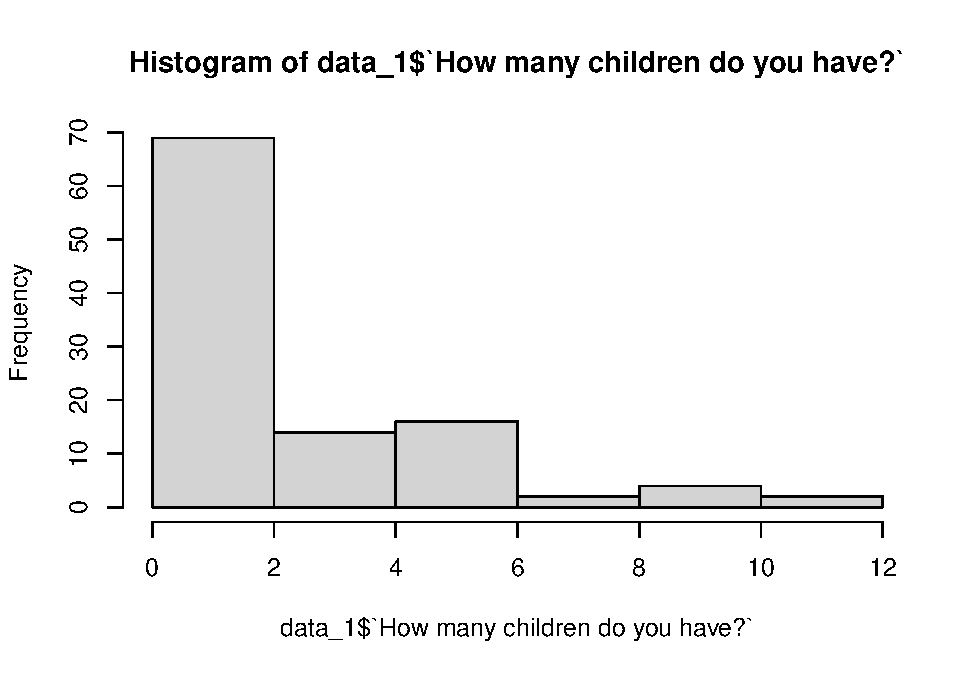
\includegraphics{04-data_manipulation_files/figure-latex/unnamed-chunk-16-1.pdf}

\begin{itemize}
\tightlist
\item
  Function boxplot(): function to plot a boxplot, it provides a compact summary of the data's central tendency, spread, and potential outliers.
\end{itemize}

\begin{Shaded}
\begin{Highlighting}[]
\FunctionTok{boxplot}\NormalTok{(data\_1}\SpecialCharTok{$}\StringTok{\textasciigrave{}}\AttributeTok{How many children do you have?}\StringTok{\textasciigrave{}}\NormalTok{)}
\end{Highlighting}
\end{Shaded}

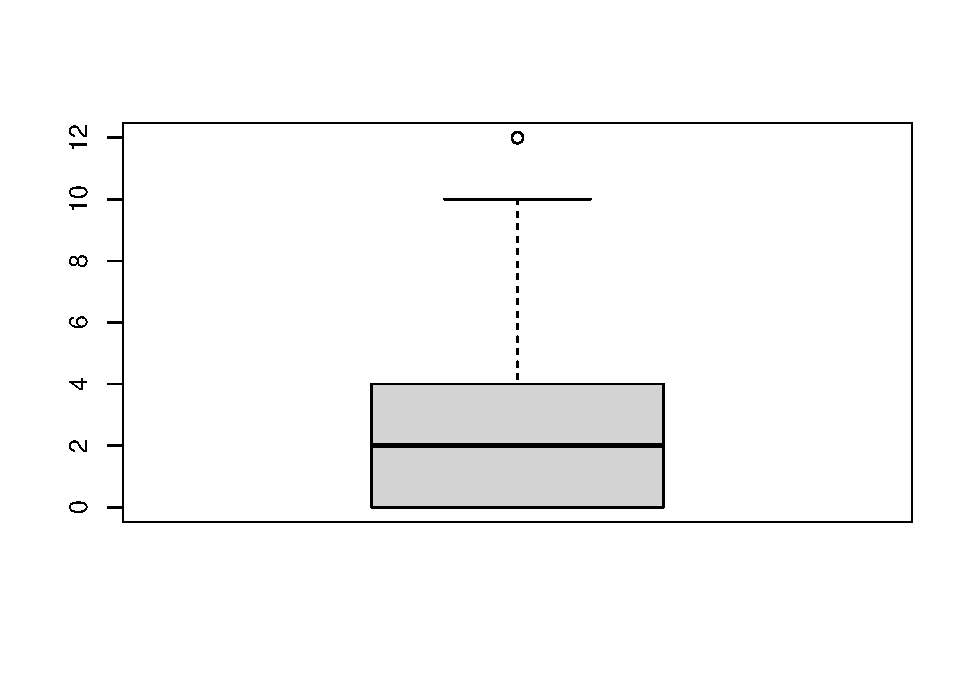
\includegraphics{04-data_manipulation_files/figure-latex/unnamed-chunk-17-1.pdf}

\hypertarget{data-manipulation-with-dplyr}{%
\section{Data manipulation with dplyr}\label{data-manipulation-with-dplyr}}

\textbf{IMPORTANT POINT:}
One of the more useful ways to use dplyr is with the pipe operator. The pipe operator looks like this: \%\textgreater\% ,and it is common practice to use the pipe operator to ``pipe'' dplyr commands together. It is a way to chain multiple operations together in a concise and precise way. The \%\textgreater\% operator takes the output of the expression on its left and passes it as the first argument to the function on its right.

In order to manipulate and clean the data, R provides a library called dplyr which consists of many built-in methods to manipulate the data. So to use the data manipulation function, first need to import the dplyr package using library(dplyr) line of code. Below is the list of fundamental data manipulation verbs that you will use to do most of your data manipulations.

\begin{itemize}
\item
  filter():

  The filter() function is used to produce the subset of the data that satisfies the condition specified in the filter() method. In the condition, we can use conditional operators, logical operators, NA values, range operators etc. to filter out data. Syntax of filter() function is given below:

\begin{verbatim}
  filter(dataframeName,condition)
\end{verbatim}
\end{itemize}

Example:

\begin{Shaded}
\begin{Highlighting}[]
\NormalTok{dplyr}\SpecialCharTok{::}\FunctionTok{filter}\NormalTok{(data\_1, Sex}\SpecialCharTok{==}\StringTok{"Female"}\NormalTok{)}
\end{Highlighting}
\end{Shaded}

\begin{itemize}
\item
  distinct():

  The distinct() method removes duplicate rows from data frame or based on the specified columns. The syntax of distinct() method is given below:

\begin{verbatim}
  distinct(dataframeName, col1, col2,.., .keep_all=TRUE)
\end{verbatim}
\end{itemize}

Example:

\begin{Shaded}
\begin{Highlighting}[]
\NormalTok{data\_1 }\SpecialCharTok{\%\textgreater{}\%} 
\NormalTok{  dplyr}\SpecialCharTok{::}\FunctionTok{distinct}\NormalTok{()}
\end{Highlighting}
\end{Shaded}

\begin{itemize}
\item
  arrange():

  In R, the arrange() method is used to order the rows based on a specified column. The syntax of arrange() method is specified below:

\begin{verbatim}
  arrange(dataframeName, columnName)
\end{verbatim}
\end{itemize}

Example:

\begin{Shaded}
\begin{Highlighting}[]
\NormalTok{data\_1 }\SpecialCharTok{\%\textgreater{}\%} 
\NormalTok{  dplyr}\SpecialCharTok{::}\FunctionTok{arrange}\NormalTok{(Sex)}
\end{Highlighting}
\end{Shaded}

\begin{itemize}
\item
  select():

  The select() method is used to extract the required columns as a table by specifying the required column names in select() method. The syntax of select() method is mentioned below:

\begin{verbatim}
  select(dataframeName, col1,col2,…)
\end{verbatim}
\end{itemize}

Example:

\begin{Shaded}
\begin{Highlighting}[]
\NormalTok{data\_1 }\SpecialCharTok{\%\textgreater{}\%} 
\NormalTok{  dplyr}\SpecialCharTok{::}\FunctionTok{select}\NormalTok{(Sex,}\StringTok{\textasciigrave{}}\AttributeTok{Do you  have children?}\StringTok{\textasciigrave{}}\NormalTok{)}
\end{Highlighting}
\end{Shaded}

\begin{itemize}
\item
  rename():

  The rename() function is used to change the column names. This can be done by the below syntax:

\begin{verbatim}
  rename(dataframeName, newName=oldName)
\end{verbatim}
\end{itemize}

Example:

\begin{Shaded}
\begin{Highlighting}[]
\NormalTok{data\_1 }\SpecialCharTok{\%\textgreater{}\%}
\NormalTok{  dplyr}\SpecialCharTok{::}\FunctionTok{rename}\NormalTok{(}\AttributeTok{Status=} \StringTok{\textasciigrave{}}\AttributeTok{Are you married?}\StringTok{\textasciigrave{}}\NormalTok{)}
\end{Highlighting}
\end{Shaded}

\begin{itemize}
\item
  mutate():

  The mutate() function creates new variables without dropping the old ones. The syntax of mutate() is specified below:

\begin{verbatim}
  mutate(dataframeName, newVariable=formula)
\end{verbatim}
\end{itemize}

Example:

\begin{Shaded}
\begin{Highlighting}[]
\NormalTok{data\_1 }\SpecialCharTok{\%\textgreater{}\%}
\NormalTok{  dplyr}\SpecialCharTok{::}\FunctionTok{mutate}\NormalTok{(}\AttributeTok{sex=}\FunctionTok{ifelse}\NormalTok{(Sex}\SpecialCharTok{==}\StringTok{"Female"}\NormalTok{, }\StringTok{"F"}\NormalTok{, }\StringTok{"M"}\NormalTok{))}
\end{Highlighting}
\end{Shaded}

\begin{itemize}
\item
  transmute():

  The transmute() function drops the old variables and creates new variables. Here is the syntax:

\begin{verbatim}
  transmute(dataframeName, newVariable=formula)
\end{verbatim}
\end{itemize}

Example:

\begin{Shaded}
\begin{Highlighting}[]
\NormalTok{data\_1 }\SpecialCharTok{\%\textgreater{}\%}
\NormalTok{  dplyr}\SpecialCharTok{::}\FunctionTok{transmute}\NormalTok{(}\AttributeTok{sex=}\FunctionTok{ifelse}\NormalTok{(Sex}\SpecialCharTok{==}\StringTok{"Female"}\NormalTok{, }\StringTok{"F"}\NormalTok{, }\StringTok{"M"}\NormalTok{))}
\end{Highlighting}
\end{Shaded}

\begin{itemize}
\item
  summarize():

  Using the summarize method we can summarize the data in the data frame by using aggregate functions like sum(), mean(), etc. Usually this function is used with the \texttt{group\_by()} function. The syntax of summarize() method is specified below:

\begin{verbatim}
  summarize(dataframeName, aggregate_function(columnName))
\end{verbatim}
\end{itemize}

Example:

\begin{Shaded}
\begin{Highlighting}[]
\NormalTok{data\_1 }\SpecialCharTok{\%\textgreater{}\%}
  \FunctionTok{group\_by}\NormalTok{(Sex) }\SpecialCharTok{\%\textgreater{}\%}
  \FunctionTok{summarize}\NormalTok{(}\AttributeTok{mean=}\FunctionTok{mean}\NormalTok{(}\StringTok{\textasciigrave{}}\AttributeTok{How many children do you have?}\StringTok{\textasciigrave{}}\NormalTok{), }\AttributeTok{count=}\FunctionTok{n}\NormalTok{())}
\end{Highlighting}
\end{Shaded}

\hypertarget{data-cleaning}{%
\chapter{Data cleaning}\label{data-cleaning}}

In the domain of data science, R reigns supreme as a tool for transforming raw data into actionable insights.
Data cleaning, a core competency of R, empowers us to clean, filter, transform, and aggregate data, paving the way for meaningful analysis. This introductory paragraph delves into the world of data manipulation and data cleaning in R, highlighting its significance and exploring the key concepts involved.

There are several methods used for data cleansing, including:

\hypertarget{renaming-colums}{%
\section{Renaming colums}\label{renaming-colums}}

During data cleansing, column renaming plays a crucial role in organizing and clarifying the dataset. This step involves assigning meaningful and consistent names to columns, which facilitates their interpretation and subsequent use in analysis.

\begin{Shaded}
\begin{Highlighting}[]
\CommentTok{\#load the package}
\FunctionTok{library}\NormalTok{(dplyr)}

\CommentTok{\#rename the variable "Are you married?"}
\NormalTok{data\_1 }\SpecialCharTok{\%\textgreater{}\%}
\NormalTok{  dplyr}\SpecialCharTok{::}\FunctionTok{rename}\NormalTok{(}\AttributeTok{marital\_status=}\StringTok{\textasciigrave{}}\AttributeTok{Are you married?}\StringTok{\textasciigrave{}}\NormalTok{)}
\end{Highlighting}
\end{Shaded}

\hypertarget{handling-missing-data}{%
\section{Handling Missing Data:}\label{handling-missing-data}}

Missing data, also known as missing values, is a common challenge encountered in data analysis. It refers to the absence of information for specific variables in certain observations within your dataset. To deal with missing data we have two options: impute data or remove data.

~~~~~~2.1) Imputation

we can use imputation by mean, median or mode.

~~~~~~~~- \emph{Imputation by mean}:

\begin{Shaded}
\begin{Highlighting}[]
\CommentTok{\#Create a new column of number of varieties}
\NormalTok{data\_1}\SpecialCharTok{$}\NormalTok{number\_variety }\OtherTok{\textless{}{-}} \FunctionTok{str\_sub}\NormalTok{(data\_1}\SpecialCharTok{$}\StringTok{\textasciigrave{}}\AttributeTok{How many varieties do you grow on the same plot or in the same field?}\StringTok{\textasciigrave{}}\NormalTok{, }\DecValTok{1}\NormalTok{, }\DecValTok{1}\NormalTok{)}

\CommentTok{\#verify the type of the column}
\FunctionTok{str}\NormalTok{(data\_1}\SpecialCharTok{$}\NormalTok{number\_variety)}

\CommentTok{\#transform the type into number}
\NormalTok{data\_1}\SpecialCharTok{$}\NormalTok{number\_variety }\OtherTok{\textless{}{-}} \FunctionTok{as.integer}\NormalTok{(data\_1}\SpecialCharTok{$}\NormalTok{number\_variety)}

\CommentTok{\#impute NA values by mean}
\NormalTok{data\_1}\SpecialCharTok{$}\NormalTok{number\_variety[}\FunctionTok{is.na}\NormalTok{(data\_1}\SpecialCharTok{$}\NormalTok{number\_variety)]}\OtherTok{\textless{}{-}}\FunctionTok{round}\NormalTok{(}\FunctionTok{mean}\NormalTok{(data\_1}\SpecialCharTok{$}\NormalTok{number\_variety, }\AttributeTok{na.rm =} \ConstantTok{TRUE}\NormalTok{))}
\end{Highlighting}
\end{Shaded}

~~~~~~~~- \emph{Imputation by median}:

\begin{Shaded}
\begin{Highlighting}[]
\FunctionTok{library}\NormalTok{(stringr)}
\CommentTok{\#function to extract the number of kg in the column}
\NormalTok{data\_1}\SpecialCharTok{$}\StringTok{\textasciigrave{}}\AttributeTok{What is the production in kg or ton/year?}\StringTok{\textasciigrave{}} \OtherTok{\textless{}{-}} \FunctionTok{sapply}\NormalTok{(data\_1}\SpecialCharTok{$}\StringTok{\textasciigrave{}}\AttributeTok{What is the production in kg or ton/year?}\StringTok{\textasciigrave{}}\NormalTok{, }\ControlFlowTok{function}\NormalTok{(x) \{}
    \CommentTok{\# Extract digits using regular expression and convert to numeric}
    \FunctionTok{str\_extract}\NormalTok{(x, }\StringTok{"}\SpecialCharTok{\textbackslash{}\textbackslash{}}\StringTok{d+"}\NormalTok{) }\SpecialCharTok{\%\textgreater{}\%} \FunctionTok{as.numeric}\NormalTok{()}
\NormalTok{\})}

\CommentTok{\#impute the column by median}
\NormalTok{data\_1}\SpecialCharTok{$}\StringTok{\textasciigrave{}}\AttributeTok{What is the production in kg or ton/year?}\StringTok{\textasciigrave{}}\NormalTok{[}\FunctionTok{is.na}\NormalTok{(data\_1}\SpecialCharTok{$}\StringTok{\textasciigrave{}}\AttributeTok{What is the production in kg or ton/year?}\StringTok{\textasciigrave{}}\NormalTok{)]}\OtherTok{\textless{}{-}}\FunctionTok{median}\NormalTok{(data\_1}\SpecialCharTok{$}\StringTok{\textasciigrave{}}\AttributeTok{What is the production in kg or ton/year?}\StringTok{\textasciigrave{}}\NormalTok{, }\AttributeTok{na.rm =} \ConstantTok{TRUE}\NormalTok{)}
\end{Highlighting}
\end{Shaded}

~~~~~~~~- \emph{Imputation by mode}:

\begin{Shaded}
\begin{Highlighting}[]
\NormalTok{data\_1}\SpecialCharTok{$}\StringTok{\textasciigrave{}}\AttributeTok{Where do you get your seeds?}\StringTok{\textasciigrave{}}\NormalTok{[}\FunctionTok{is.na}\NormalTok{(data\_1}\SpecialCharTok{$}\StringTok{\textasciigrave{}}\AttributeTok{Where do you get your seeds?}\StringTok{\textasciigrave{}}\NormalTok{)] }\OtherTok{\textless{}{-}} \FunctionTok{names}\NormalTok{(}\FunctionTok{which.max}\NormalTok{(}\FunctionTok{table}\NormalTok{(data\_1}\SpecialCharTok{$}\StringTok{\textasciigrave{}}\AttributeTok{Where do you get your seeds?}\StringTok{\textasciigrave{}}\NormalTok{)))}
\end{Highlighting}
\end{Shaded}

~~~~~~2.2) Removing data

There are 2 usuals methods for deleting data when dealing with missing data: listwise and dropping variables.

~~~~~~~~- \emph{Listwise}:

In this method, all data for an observation that has one or more missing values are deleted. The analysis is run only on observations that have a complete set of data.

\begin{Shaded}
\begin{Highlighting}[]
\FunctionTok{na.omit}\NormalTok{(data\_1)}
\end{Highlighting}
\end{Shaded}

~~~~~~~~- \emph{Dropping variables}:

If data is missing for a large proportion of the observations, it may be best to discard the variable entirely if it is insignificant.

\begin{Shaded}
\begin{Highlighting}[]
\FunctionTok{subset}\NormalTok{( data\_1, }\AttributeTok{select =} \SpecialCharTok{{-}}\FunctionTok{c}\NormalTok{(}\StringTok{\textasciigrave{}}\AttributeTok{How do you call these varieties you have?}\StringTok{\textasciigrave{}}\NormalTok{))}
\end{Highlighting}
\end{Shaded}

\hypertarget{handling-outliers}{%
\section{Handling outliers}\label{handling-outliers}}

Data points far from the dataset's other points are considered outliers. The presence of outliers can pose significant problems in statistical analysis and machine learning. They can bias model parameter estimates, lead to erroneous conclusions and affect algorithm performance.

\begin{Shaded}
\begin{Highlighting}[]
\NormalTok{outlier\_values }\OtherTok{\textless{}{-}} \FunctionTok{boxplot.stats}\NormalTok{(data\_1}\SpecialCharTok{$}\StringTok{\textasciigrave{}}\AttributeTok{How many children do you have?}\StringTok{\textasciigrave{}}\NormalTok{)}\SpecialCharTok{$}\NormalTok{out  }\CommentTok{\# outlier values.}
\FunctionTok{boxplot}\NormalTok{(data\_1}\SpecialCharTok{$}\StringTok{\textasciigrave{}}\AttributeTok{How many children do you have?}\StringTok{\textasciigrave{}}\NormalTok{, }\AttributeTok{main=}\StringTok{"Number of children"}\NormalTok{, }\AttributeTok{boxwex=}\FloatTok{0.1}\NormalTok{)}
\FunctionTok{mtext}\NormalTok{(}\FunctionTok{paste}\NormalTok{(}\StringTok{"Outliers: "}\NormalTok{, }\FunctionTok{paste}\NormalTok{(outlier\_values, }\AttributeTok{collapse=}\StringTok{", "}\NormalTok{)), }\AttributeTok{cex=}\FloatTok{0.6}\NormalTok{)}
\end{Highlighting}
\end{Shaded}

After identify outliers you can handle it by either impute those outliers by a value (mean, median, mode) or use the method of capping (For missing values that lie outside the **1.5 * IQR** limits, we could cap it by replacing those observations outside the lower limit with the value of 5th percentile and those that lie above the upper limit, with the value of 95th percentile)

\hypertarget{removing-duplicates}{%
\section{\texorpdfstring{Removing duplicates:\\
}{Removing duplicates: }}\label{removing-duplicates}}

Removing duplicates ensures that each data point is represented only once, leading to more accurate and consistent data for analysis.

\begin{Shaded}
\begin{Highlighting}[]
\NormalTok{data\_1 }\OtherTok{\textless{}{-}}\NormalTok{ data\_1 }\SpecialCharTok{\%\textgreater{}\%} 
\NormalTok{  dplyr}\SpecialCharTok{::}\FunctionTok{distinct}\NormalTok{()}
\end{Highlighting}
\end{Shaded}

\hypertarget{checking-data-structure}{%
\section{Checking data structure:}\label{checking-data-structure}}

Checking data types is a crucial step in data analysis because it ensures you're working with the data in the way it's intended in order to avoid errors later in the analysis.

\begin{Shaded}
\begin{Highlighting}[]
\FunctionTok{str}\NormalTok{(data\_1)}
\end{Highlighting}
\end{Shaded}

You can change the type of your data across many functions like: as.numeric(), as.character(), as.factor() etc\ldots.if the data is not in the right type.

\hypertarget{handling-inconsistent-categorical-data}{%
\section{Handling Inconsistent Categorical Data}\label{handling-inconsistent-categorical-data}}

Categorical variables may have inconsistent spellings or categories. The recode() function or manual recoding can help standardize categories.

\begin{Shaded}
\begin{Highlighting}[]
\NormalTok{data\_1 }\OtherTok{\textless{}{-}}\NormalTok{ data\_1 }\SpecialCharTok{\%\textgreater{}\%}
\NormalTok{  dplyr}\SpecialCharTok{::}\FunctionTok{mutate}\NormalTok{(}\StringTok{\textasciigrave{}}\AttributeTok{How do you store your seed?}\StringTok{\textasciigrave{}} \OtherTok{=}\NormalTok{ dplyr}\SpecialCharTok{::}\FunctionTok{recode}\NormalTok{(}\StringTok{\textasciigrave{}}\AttributeTok{How do you store your seed?}\StringTok{\textasciigrave{}}\NormalTok{, }\StringTok{"In bags"} \OtherTok{=} \StringTok{"in bags"}\NormalTok{))}
\end{Highlighting}
\end{Shaded}

\hypertarget{combine-dataframes}{%
\section{Combine dataframes}\label{combine-dataframes}}

Suppose the dataset combines data from different sources, we can combine differents datasets into one. When combining data from multiple sources, ensure that all data fields align correctly.
~~~~- Combine by column

\begin{Shaded}
\begin{Highlighting}[]
\NormalTok{culture1 }\OtherTok{\textless{}{-}} \FunctionTok{data.frame}\NormalTok{(}
  \AttributeTok{Culture =} \FunctionTok{c}\NormalTok{(}\StringTok{"wheat"}\NormalTok{, }\StringTok{"maize"}\NormalTok{, }\StringTok{"rice"}\NormalTok{),}
  \AttributeTok{Area =} \FunctionTok{c}\NormalTok{(}\DecValTok{100}\NormalTok{, }\DecValTok{150}\NormalTok{, }\DecValTok{120}\NormalTok{)}
\NormalTok{)}

\NormalTok{culture2 }\OtherTok{\textless{}{-}} \FunctionTok{data.frame}\NormalTok{(}
  \AttributeTok{Culture =} \FunctionTok{c}\NormalTok{(}\StringTok{"wheat"}\NormalTok{, }\StringTok{"maize"}\NormalTok{, }\StringTok{"rice"}\NormalTok{),}
  \AttributeTok{Return =} \FunctionTok{c}\NormalTok{(}\DecValTok{50}\NormalTok{, }\DecValTok{60}\NormalTok{, }\DecValTok{45}\NormalTok{)}
\NormalTok{)}

\NormalTok{culture\_final1 }\OtherTok{\textless{}{-}} \FunctionTok{cbind}\NormalTok{(culture1, culture2)}
\end{Highlighting}
\end{Shaded}

~~~~- combine by row

\begin{Shaded}
\begin{Highlighting}[]
\NormalTok{culture3 }\OtherTok{\textless{}{-}} \FunctionTok{data.frame}\NormalTok{(}
  \AttributeTok{Culture =} \FunctionTok{c}\NormalTok{(}\StringTok{"wheat"}\NormalTok{, }\StringTok{"maize"}\NormalTok{, }\StringTok{"rice"}\NormalTok{),}
  \AttributeTok{Area =} \FunctionTok{c}\NormalTok{(}\DecValTok{100}\NormalTok{, }\DecValTok{150}\NormalTok{, }\DecValTok{120}\NormalTok{)}
\NormalTok{)}

\NormalTok{culture4 }\OtherTok{\textless{}{-}} \FunctionTok{data.frame}\NormalTok{(}
  \AttributeTok{Culture =} \FunctionTok{c}\NormalTok{(}\StringTok{"potato"}\NormalTok{, }\StringTok{"cassava"}\NormalTok{),}
  \AttributeTok{Area =} \FunctionTok{c}\NormalTok{(}\DecValTok{250}\NormalTok{, }\DecValTok{400}\NormalTok{)}
\NormalTok{)}

\NormalTok{culture\_final2 }\OtherTok{\textless{}{-}} \FunctionTok{rbind}\NormalTok{(culture3, culture4)}
\end{Highlighting}
\end{Shaded}

\hypertarget{data-validation}{%
\section{Data Validation}\label{data-validation}}

Data validation involves checking data against predefined rules or criteria. It ensures that data adheres to specific requirements or constraints.

Validation checks can prevent incorrect or inconsistent data from entering your analysis.

\hypertarget{regular-expressions}{%
\section{Regular expressions}\label{regular-expressions}}

Regular expressions (regex) are powerful tools for pattern matching and replacement in text data. The gsub() function is commonly used for global pattern substitution.

\begin{Shaded}
\begin{Highlighting}[]
\NormalTok{data\_1}\SpecialCharTok{$}\StringTok{\textasciigrave{}}\AttributeTok{How much does 1kg of tasba seed cost?}\StringTok{\textasciigrave{}} \OtherTok{\textless{}{-}} \FunctionTok{gsub}\NormalTok{(}\StringTok{"FCFA"}\NormalTok{, }\StringTok{""}\NormalTok{, }
\NormalTok{                        data\_1}\SpecialCharTok{$}\StringTok{\textasciigrave{}}\AttributeTok{How much does 1kg of tasba seed cost?}\StringTok{\textasciigrave{}}\NormalTok{)}
\end{Highlighting}
\end{Shaded}

\begin{Shaded}
\begin{Highlighting}[]
\NormalTok{knitr}\SpecialCharTok{::}\FunctionTok{knit\_child}\NormalTok{(}\StringTok{"05{-}data\_cleaning.Rmd"}\NormalTok{)}
\CommentTok{\#\textgreater{} }
\CommentTok{\#\textgreater{} }
\CommentTok{\#\textgreater{} processing file: ./05{-}data\_cleaning.Rmd}
\CommentTok{\#\textgreater{} }
  \SpecialCharTok{|}                                     
  \ErrorTok{|}                               \ErrorTok{|}   \DecValTok{0}\NormalTok{\%}
  \SpecialCharTok{|}                                     
  \ErrorTok{|}\NormalTok{.                              }\SpecialCharTok{|}   \DecValTok{4}\NormalTok{\% [unnamed}\SpecialCharTok{{-}}\NormalTok{chunk}\DecValTok{{-}13}\NormalTok{]}
  \SpecialCharTok{|}                                     
  \ErrorTok{|}\NormalTok{..                             }\SpecialCharTok{|}   \DecValTok{7}\NormalTok{\%                   }
  \SpecialCharTok{|}                                     
  \ErrorTok{|}\NormalTok{...                            }\SpecialCharTok{|}  \DecValTok{11}\NormalTok{\% [unnamed}\SpecialCharTok{{-}}\NormalTok{chunk}\DecValTok{{-}14}\NormalTok{]}
  \SpecialCharTok{|}                                     
  \ErrorTok{|}\NormalTok{....                           }\SpecialCharTok{|}  \DecValTok{14}\NormalTok{\%                   }
  \SpecialCharTok{|}                                     
  \ErrorTok{|}\NormalTok{......                         }\SpecialCharTok{|}  \DecValTok{18}\NormalTok{\% [unnamed}\SpecialCharTok{{-}}\NormalTok{chunk}\DecValTok{{-}15}\NormalTok{]}
  \SpecialCharTok{|}                                     
  \ErrorTok{|}\NormalTok{.......                        }\SpecialCharTok{|}  \DecValTok{21}\NormalTok{\%                   }
  \SpecialCharTok{|}                                     
  \ErrorTok{|}\NormalTok{........                       }\SpecialCharTok{|}  \DecValTok{25}\NormalTok{\% [unnamed}\SpecialCharTok{{-}}\NormalTok{chunk}\DecValTok{{-}16}\NormalTok{]}
  \SpecialCharTok{|}                                     
  \ErrorTok{|}\NormalTok{.........                      }\SpecialCharTok{|}  \DecValTok{29}\NormalTok{\%                   }
  \SpecialCharTok{|}                                     
  \ErrorTok{|}\NormalTok{..........                     }\SpecialCharTok{|}  \DecValTok{32}\NormalTok{\% [unnamed}\SpecialCharTok{{-}}\NormalTok{chunk}\DecValTok{{-}17}\NormalTok{]}
  \SpecialCharTok{|}                                     
  \ErrorTok{|}\NormalTok{...........                    }\SpecialCharTok{|}  \DecValTok{36}\NormalTok{\%                   }
  \SpecialCharTok{|}                                     
  \ErrorTok{|}\NormalTok{............                   }\SpecialCharTok{|}  \DecValTok{39}\NormalTok{\% [unnamed}\SpecialCharTok{{-}}\NormalTok{chunk}\DecValTok{{-}18}\NormalTok{]}
  \SpecialCharTok{|}                                     
  \ErrorTok{|}\NormalTok{.............                  }\SpecialCharTok{|}  \DecValTok{43}\NormalTok{\%                   }
  \SpecialCharTok{|}                                     
  \ErrorTok{|}\NormalTok{..............                 }\SpecialCharTok{|}  \DecValTok{46}\NormalTok{\% [unnamed}\SpecialCharTok{{-}}\NormalTok{chunk}\DecValTok{{-}19}\NormalTok{]}
  \SpecialCharTok{|}                                     
  \ErrorTok{|}\NormalTok{................               }\SpecialCharTok{|}  \DecValTok{50}\NormalTok{\%                   }
  \SpecialCharTok{|}                                     
  \ErrorTok{|}\NormalTok{.................              }\SpecialCharTok{|}  \DecValTok{54}\NormalTok{\% [unnamed}\SpecialCharTok{{-}}\NormalTok{chunk}\DecValTok{{-}20}\NormalTok{]}
  \SpecialCharTok{|}                                     
  \ErrorTok{|}\NormalTok{..................             }\SpecialCharTok{|}  \DecValTok{57}\NormalTok{\%                   }
  \SpecialCharTok{|}                                     
  \ErrorTok{|}\NormalTok{...................            }\SpecialCharTok{|}  \DecValTok{61}\NormalTok{\% [unnamed}\SpecialCharTok{{-}}\NormalTok{chunk}\DecValTok{{-}21}\NormalTok{]}
  \SpecialCharTok{|}                                     
  \ErrorTok{|}\NormalTok{....................           }\SpecialCharTok{|}  \DecValTok{64}\NormalTok{\%                   }
  \SpecialCharTok{|}                                     
  \ErrorTok{|}\NormalTok{.....................          }\SpecialCharTok{|}  \DecValTok{68}\NormalTok{\% [unnamed}\SpecialCharTok{{-}}\NormalTok{chunk}\DecValTok{{-}22}\NormalTok{]}
  \SpecialCharTok{|}                                     
  \ErrorTok{|}\NormalTok{......................         }\SpecialCharTok{|}  \DecValTok{71}\NormalTok{\%                   }
  \SpecialCharTok{|}                                     
  \ErrorTok{|}\NormalTok{.......................        }\SpecialCharTok{|}  \DecValTok{75}\NormalTok{\% [unnamed}\SpecialCharTok{{-}}\NormalTok{chunk}\DecValTok{{-}23}\NormalTok{]}
  \SpecialCharTok{|}                                     
  \ErrorTok{|}\NormalTok{........................       }\SpecialCharTok{|}  \DecValTok{79}\NormalTok{\%                   }
  \SpecialCharTok{|}                                     
  \ErrorTok{|}\NormalTok{.........................      }\SpecialCharTok{|}  \DecValTok{82}\NormalTok{\% [unnamed}\SpecialCharTok{{-}}\NormalTok{chunk}\DecValTok{{-}24}\NormalTok{]}
  \SpecialCharTok{|}                                     
  \ErrorTok{|}\NormalTok{...........................    }\SpecialCharTok{|}  \DecValTok{86}\NormalTok{\%                   }
  \SpecialCharTok{|}                                     
  \ErrorTok{|}\NormalTok{............................   }\SpecialCharTok{|}  \DecValTok{89}\NormalTok{\% [unnamed}\SpecialCharTok{{-}}\NormalTok{chunk}\DecValTok{{-}25}\NormalTok{]}
  \SpecialCharTok{|}                                     
  \ErrorTok{|}\NormalTok{.............................  }\SpecialCharTok{|}  \DecValTok{93}\NormalTok{\%                   }
  \SpecialCharTok{|}                                     
  \ErrorTok{|}\NormalTok{.............................. }\SpecialCharTok{|}  \DecValTok{96}\NormalTok{\% [unnamed}\SpecialCharTok{{-}}\NormalTok{chunk}\DecValTok{{-}26}\NormalTok{]}
  \SpecialCharTok{|}                                     
  \ErrorTok{|}\NormalTok{...............................}\SpecialCharTok{|} \DecValTok{100}\NormalTok{\%                   }
\end{Highlighting}
\end{Shaded}

\begin{verbatim}
#> [1] "\n\n\n# Data cleaning\n\nIn the domain of data science, R reigns supreme as a tool for transforming raw data into actionable insights. \nData cleaning, a core competency of R, empowers us to clean, filter, transform, and aggregate data, paving the way for meaningful analysis. This introductory paragraph delves into the world of data manipulation and data cleaning in R, highlighting its significance and exploring the key concepts involved.\n\nThere are several methods used for data cleansing, including:\n\n## Renaming colums\n\nDuring data cleansing, column renaming plays a crucial role in organizing and clarifying the dataset. This step involves assigning meaningful and consistent names to columns, which facilitates their interpretation and subsequent use in analysis.\n\n\n```r\n#load the package\nlibrary(dplyr)\n\n#rename the variable \"Are you married?\"\ndata_1 %>%\n  dplyr::rename(marital_status=`Are you married?`)\n```\n\n\n## Handling Missing Data: \n\nMissing data, also known as missing values, is a common challenge encountered in data analysis. It refers to the absence of information for specific variables in certain observations within your dataset. To deal with missing data we have two options: impute data or remove data.\n\n&nbsp;&nbsp;&nbsp;&nbsp;&nbsp;&nbsp;2.1) Imputation\n\nwe can use imputation by mean, median or mode.\n\n&nbsp;&nbsp;&nbsp;&nbsp;&nbsp;&nbsp;&nbsp;&nbsp;- *Imputation by mean*:\n\n\n```r\n#Create a new column of number of varieties\ndata_1$number_variety <- str_sub(data_1$`How many varieties do you grow on the same plot or in the same field?`, 1, 1)\n\n#verify the type of the column\nstr(data_1$number_variety)\n\n#transform the type into number\ndata_1$number_variety <- as.integer(data_1$number_variety)\n\n#impute NA values by mean\ndata_1$number_variety[is.na(data_1$number_variety)]<-round(mean(data_1$number_variety, na.rm = TRUE))\n```\n\n\n&nbsp;&nbsp;&nbsp;&nbsp;&nbsp;&nbsp;&nbsp;&nbsp;- *Imputation by median*:\n\n\n```r\nlibrary(stringr)\n#function to extract the number of kg in the column\ndata_1$`What is the production in kg or ton/year?` <- sapply(data_1$`What is the production in kg or ton/year?`, function(x) {\n    # Extract digits using regular expression and convert to numeric\n    str_extract(x, \"\\\\d+\") %>% as.numeric()\n})\n\n#impute the column by median\ndata_1$`What is the production in kg or ton/year?`[is.na(data_1$`What is the production in kg or ton/year?`)]<-median(data_1$`What is the production in kg or ton/year?`, na.rm = TRUE)\n\n```\n\n\n&nbsp;&nbsp;&nbsp;&nbsp;&nbsp;&nbsp;&nbsp;&nbsp;- *Imputation by mode*:\n\n\n```r\ndata_1$`Where do you get your seeds?`[is.na(data_1$`Where do you get your seeds?`)] <- names(which.max(table(data_1$`Where do you get your seeds?`)))\n```\n\n&nbsp;&nbsp;&nbsp;&nbsp;&nbsp;&nbsp;2.2) Removing data\n\nThere are 2 usuals methods for deleting data when dealing with missing data: listwise and dropping variables.\n\n&nbsp;&nbsp;&nbsp;&nbsp;&nbsp;&nbsp;&nbsp;&nbsp;- *Listwise*:\n\nIn this method, all data for an observation that has one or more missing values are deleted. The analysis is run only on observations that have a complete set of data. \n\n\n```r\nna.omit(data_1)\n```\n\n\n&nbsp;&nbsp;&nbsp;&nbsp;&nbsp;&nbsp;&nbsp;&nbsp;- *Dropping variables*:\n\nIf data is missing for a large proportion of the observations, it may be best to discard the variable entirely if it is insignificant.\n\n\n```r\nsubset( data_1, select = -c(`How do you call these varieties you have?`))\n```\n\n## Handling outliers\n\nData points far from the dataset’s other points are considered outliers. The presence of outliers can pose significant problems in statistical analysis and machine learning. They can bias model parameter estimates, lead to erroneous conclusions and affect algorithm performance.\n\n\n```r\noutlier_values <- boxplot.stats(data_1$`How many children do you have?`)$out  # outlier values.\nboxplot(data_1$`How many children do you have?`, main=\"Number of children\", boxwex=0.1)\nmtext(paste(\"Outliers: \", paste(outlier_values, collapse=\", \")), cex=0.6)\n```\n\nAfter identify outliers you can handle it by either impute those outliers by a value (mean, median, mode) or use the method of capping (For missing values that lie outside the **1.5 * IQR** limits, we could cap it by replacing those observations outside the lower limit with the value of 5th percentile and those that lie above the upper limit, with the value of 95th percentile)\n\n## Removing duplicates: \\\nRemoving duplicates ensures that each data point is represented only once, leading to more accurate and consistent data for analysis.\n\n\n```r\ndata_1 <- data_1 %>% \n  dplyr::distinct()\n```\n\n## Checking data structure: \n\nChecking data types is a crucial step in data analysis because it ensures you're working with the data in the way it's intended in order to avoid errors later in the analysis.\n\n\n```r\nstr(data_1)\n```\n\nYou can change the type of your data across many functions like: as.numeric(), as.character(), as.factor() etc....if the data is not in the right type.\n\n## Handling Inconsistent Categorical Data\n\nCategorical variables may have inconsistent spellings or categories. The recode() function or manual recoding can help standardize categories.\n\n\n```r\ndata_1 <- data_1 %>%\n  dplyr::mutate(`How do you store your seed?` = dplyr::recode(`How do you store your seed?`, \"In bags\" = \"in bags\"))\n```\n\n\n## Combine dataframes\n\nSuppose the dataset combines data from different sources, we can combine differents datasets into one. When combining data from multiple sources, ensure that all data fields align correctly.\n&nbsp;&nbsp;&nbsp;&nbsp;- Combine by column\n\n\n```r\nculture1 <- data.frame(\n  Culture = c(\"wheat\", \"maize\", \"rice\"),\n  Area = c(100, 150, 120)\n)\n\nculture2 <- data.frame(\n  Culture = c(\"wheat\", \"maize\", \"rice\"),\n  Return = c(50, 60, 45)\n)\n\nculture_final1 <- cbind(culture1, culture2)\n```\n\n&nbsp;&nbsp;&nbsp;&nbsp;- combine by row\n\n\n```r\nculture3 <- data.frame(\n  Culture = c(\"wheat\", \"maize\", \"rice\"),\n  Area = c(100, 150, 120)\n)\n\nculture4 <- data.frame(\n  Culture = c(\"potato\", \"cassava\"),\n  Area = c(250, 400)\n)\n\nculture_final2 <- rbind(culture3, culture4)\n```\n\n## Data Validation\n\nData validation involves checking data against predefined rules or criteria. It ensures that data adheres to specific requirements or constraints.\n\nValidation checks can prevent incorrect or inconsistent data from entering your analysis.\n\n## Regular expressions\n\nRegular expressions (regex) are powerful tools for pattern matching and replacement in text data. The gsub() function is commonly used for global pattern substitution.\n\n\n```r\ndata_1$`How much does 1kg of tasba seed cost?` <- gsub(\"FCFA\", \"\", \n                        data_1$`How much does 1kg of tasba seed cost?`)\n```\n\n\n"
\end{verbatim}

\begin{Shaded}
\begin{Highlighting}[]
\FunctionTok{source}\NormalTok{(}\StringTok{"./dependencies.R"}\NormalTok{)}
\end{Highlighting}
\end{Shaded}

\hypertarget{descriptive-statistics}{%
\chapter{Descriptive statistics}\label{descriptive-statistics}}

\hypertarget{central-tendency-indicators}{%
\section{Central Tendency Indicators}\label{central-tendency-indicators}}

Central tendency indicators, also known as measures of central tendency, are statistical measures used to summarize a set of data by finding a single value that represents the middle or center of that data. They basically give you an idea of where most of the data points tend to cluster around.

There are three main types of central tendency indicators:

\begin{enumerate}
\def\labelenumi{\arabic{enumi}.}
\tightlist
\item
  Mean\\
  This is the most common one, also called the average. It's calculated by adding up all the values in your data set and then dividing by the number of values.\\
\end{enumerate}

\begin{Shaded}
\begin{Highlighting}[]
\FunctionTok{mean}\NormalTok{(data\_1}\SpecialCharTok{$}\StringTok{\textasciigrave{}}\AttributeTok{What is the production in kg or ton/year?}\StringTok{\textasciigrave{}}\NormalTok{)}
\CommentTok{\#\textgreater{} [1] 138.3084}
\end{Highlighting}
\end{Shaded}

\begin{enumerate}
\def\labelenumi{\arabic{enumi}.}
\setcounter{enumi}{1}
\tightlist
\item
  Median\\
  This is the middle number when you arrange your data set in order, from least to greatest. If you have an even number of data points, the median is the average of the two middle numbers.\\
\end{enumerate}

\begin{Shaded}
\begin{Highlighting}[]
\FunctionTok{median}\NormalTok{(data\_1}\SpecialCharTok{$}\StringTok{\textasciigrave{}}\AttributeTok{What is the production in kg or ton/year?}\StringTok{\textasciigrave{}}\NormalTok{)}
\CommentTok{\#\textgreater{} [1] 8}
\end{Highlighting}
\end{Shaded}

\begin{enumerate}
\def\labelenumi{\arabic{enumi}.}
\setcounter{enumi}{2}
\tightlist
\item
  Mode\\
  This is the most frequent value in your data set. You can have multiple modes, by the way, if there are a couple of values that tie for the most frequent.
\end{enumerate}

\begin{Shaded}
\begin{Highlighting}[]
\FunctionTok{names}\NormalTok{(}\FunctionTok{which.max}\NormalTok{(}\FunctionTok{table}\NormalTok{(data\_1}\SpecialCharTok{$}\StringTok{\textasciigrave{}}\AttributeTok{Are you married?}\StringTok{\textasciigrave{}}\NormalTok{)))}
\CommentTok{\#\textgreater{} [1] "YES"}
\end{Highlighting}
\end{Shaded}

\hypertarget{variability-indicators}{%
\section{Variability indicators}\label{variability-indicators}}

Variability indicators, in contrast to central tendency, tell you how spread out your data is. They describe how much the data points differ from each other and from the central value (mean, median, or mode). There are a few common ways to measure variability:

\begin{enumerate}
\def\labelenumi{\arabic{enumi}.}
\tightlist
\item
  Variance\\
  This is the average of the squared deviations of each data point from the mean. It tells you how much your data varies on average, but since it uses squared values, it can be sensitive to extreme values.
\end{enumerate}

\begin{Shaded}
\begin{Highlighting}[]
\FunctionTok{var}\NormalTok{(data\_1}\SpecialCharTok{$}\StringTok{\textasciigrave{}}\AttributeTok{What is the production in kg or ton/year?}\StringTok{\textasciigrave{}}\NormalTok{)}
\CommentTok{\#\textgreater{} [1] 296798.9}
\end{Highlighting}
\end{Shaded}

\begin{enumerate}
\def\labelenumi{\arabic{enumi}.}
\setcounter{enumi}{1}
\tightlist
\item
  Standard deviation\\
  This is the square root of the variance. Standard deviation is expressed in the same units as your original data (e.g., meters, dollars), which can be easier to interpret than variance. It also reflects how much your data deviates from the mean on average.
\end{enumerate}

\begin{Shaded}
\begin{Highlighting}[]
\CommentTok{\#1st approch using the native function}
\FunctionTok{sd}\NormalTok{(data\_1}\SpecialCharTok{$}\StringTok{\textasciigrave{}}\AttributeTok{What is the production in kg or ton/year?}\StringTok{\textasciigrave{}}\NormalTok{)}
\CommentTok{\#\textgreater{} [1] 544.7925}

\CommentTok{\#2nd approch}
\FunctionTok{sqrt}\NormalTok{(}\FunctionTok{var}\NormalTok{(data\_1}\SpecialCharTok{$}\StringTok{\textasciigrave{}}\AttributeTok{What is the production in kg or ton/year?}\StringTok{\textasciigrave{}}\NormalTok{))}
\CommentTok{\#\textgreater{} [1] 544.7925}
\end{Highlighting}
\end{Shaded}

\begin{enumerate}
\def\labelenumi{\arabic{enumi}.}
\setcounter{enumi}{2}
\tightlist
\item
  Range\\
  This is the simplest method. It's just the difference between the highest and lowest values in your data set. While easy to calculate, the range can be misleading if your data has outliers.
\end{enumerate}

\begin{Shaded}
\begin{Highlighting}[]
\FunctionTok{max}\NormalTok{(data\_1}\SpecialCharTok{$}\StringTok{\textasciigrave{}}\AttributeTok{How many children do you have?}\StringTok{\textasciigrave{}}\NormalTok{) }\SpecialCharTok{{-}} \FunctionTok{min}\NormalTok{(data\_1}\SpecialCharTok{$}\StringTok{\textasciigrave{}}\AttributeTok{How many children do you have?}\StringTok{\textasciigrave{}}\NormalTok{)}
\CommentTok{\#\textgreater{} [1] 12}
\end{Highlighting}
\end{Shaded}

\begin{enumerate}
\def\labelenumi{\arabic{enumi}.}
\setcounter{enumi}{3}
\tightlist
\item
  Interquartile range (IQR)\\
  This focuses on the middle half of your data. It represents the range between the first quartile (Q1) and the third quartile (Q3). Half your data falls within this IQR, giving a better idea of how spread out the bulk of the data is.
\end{enumerate}

\begin{Shaded}
\begin{Highlighting}[]
\FunctionTok{IQR}\NormalTok{(data\_1}\SpecialCharTok{$}\StringTok{\textasciigrave{}}\AttributeTok{How many children do you have?}\StringTok{\textasciigrave{}}\NormalTok{)}
\CommentTok{\#\textgreater{} [1] 4}
\end{Highlighting}
\end{Shaded}

\hypertarget{quantiles}{%
\section{Quantiles}\label{quantiles}}

Quantiles are values that split sorted data or a probability distribution into equal parts. In general terms, a q-quantile divides sorted data into q parts. The most commonly used quantiles have special names:

~~~~~~Quartiles:

\begin{Shaded}
\begin{Highlighting}[]
\FunctionTok{quantile}\NormalTok{(data\_1}\SpecialCharTok{$}\StringTok{\textasciigrave{}}\AttributeTok{How many children do you have?}\StringTok{\textasciigrave{}}\NormalTok{)}
\CommentTok{\#\textgreater{}   0\%  25\%  50\%  75\% 100\% }
\CommentTok{\#\textgreater{}    0    0    2    4   12}
\end{Highlighting}
\end{Shaded}

~~~~~~Deciles:

\begin{Shaded}
\begin{Highlighting}[]
\FunctionTok{quantile}\NormalTok{(data\_1}\SpecialCharTok{$}\StringTok{\textasciigrave{}}\AttributeTok{How many children do you have?}\StringTok{\textasciigrave{}}\NormalTok{,}\AttributeTok{probs =} \FunctionTok{seq}\NormalTok{(}\DecValTok{0}\NormalTok{, }\DecValTok{1}\NormalTok{, }\AttributeTok{by =} \FloatTok{0.1}\NormalTok{))}
\CommentTok{\#\textgreater{}   0\%  10\%  20\%  30\%  40\%  50\%  60\%  70\%  80\%  90\% 100\% }
\CommentTok{\#\textgreater{}    0    0    0    0    0    2    2    3    5    6   12}
\end{Highlighting}
\end{Shaded}

~~~~~~Percentiles:

\begin{Shaded}
\begin{Highlighting}[]
\FunctionTok{quantile}\NormalTok{(data\_1}\SpecialCharTok{$}\StringTok{\textasciigrave{}}\AttributeTok{How many children do you have?}\StringTok{\textasciigrave{}}\NormalTok{,}\AttributeTok{probs =} \FunctionTok{seq}\NormalTok{(}\DecValTok{0}\NormalTok{, }\DecValTok{1}\NormalTok{, }\AttributeTok{by =} \FloatTok{0.01}\NormalTok{))}
\CommentTok{\#\textgreater{}    0\%    1\%    2\%    3\%    4\%    5\%    6\%    7\%    8\%    9\% }
\CommentTok{\#\textgreater{}  0.00  0.00  0.00  0.00  0.00  0.00  0.00  0.00  0.00  0.00 }
\CommentTok{\#\textgreater{}   10\%   11\%   12\%   13\%   14\%   15\%   16\%   17\%   18\%   19\% }
\CommentTok{\#\textgreater{}  0.00  0.00  0.00  0.00  0.00  0.00  0.00  0.00  0.00  0.00 }
\CommentTok{\#\textgreater{}   20\%   21\%   22\%   23\%   24\%   25\%   26\%   27\%   28\%   29\% }
\CommentTok{\#\textgreater{}  0.00  0.00  0.00  0.00  0.00  0.00  0.00  0.00  0.00  0.00 }
\CommentTok{\#\textgreater{}   30\%   31\%   32\%   33\%   34\%   35\%   36\%   37\%   38\%   39\% }
\CommentTok{\#\textgreater{}  0.00  0.00  0.00  0.00  0.00  0.00  0.00  0.00  0.00  0.00 }
\CommentTok{\#\textgreater{}   40\%   41\%   42\%   43\%   44\%   45\%   46\%   47\%   48\%   49\% }
\CommentTok{\#\textgreater{}  0.00  0.46  1.00  1.00  1.00  1.00  1.00  1.00  1.88  2.00 }
\CommentTok{\#\textgreater{}   50\%   51\%   52\%   53\%   54\%   55\%   56\%   57\%   58\%   59\% }
\CommentTok{\#\textgreater{}  2.00  2.00  2.00  2.00  2.00  2.00  2.00  2.00  2.00  2.00 }
\CommentTok{\#\textgreater{}   60\%   61\%   62\%   63\%   64\%   65\%   66\%   67\%   68\%   69\% }
\CommentTok{\#\textgreater{}  2.00  2.00  2.00  2.00  2.00  2.90  3.00  3.00  3.00  3.00 }
\CommentTok{\#\textgreater{}   70\%   71\%   72\%   73\%   74\%   75\%   76\%   77\%   78\%   79\% }
\CommentTok{\#\textgreater{}  3.00  3.00  3.00  3.38  4.00  4.00  4.00  4.00  4.68  5.00 }
\CommentTok{\#\textgreater{}   80\%   81\%   82\%   83\%   84\%   85\%   86\%   87\%   88\%   89\% }
\CommentTok{\#\textgreater{}  5.00  5.00  5.00  5.00  5.00  5.00  5.00  5.00  5.28  6.00 }
\CommentTok{\#\textgreater{}   90\%   91\%   92\%   93\%   94\%   95\%   96\%   97\%   98\%   99\% }
\CommentTok{\#\textgreater{}  6.00  6.00  6.00  6.58  7.64  8.70  9.76 10.00 10.00 11.88 }
\CommentTok{\#\textgreater{}  100\% }
\CommentTok{\#\textgreater{} 12.00}
\end{Highlighting}
\end{Shaded}

\hypertarget{contingency-table}{%
\section{Contingency table}\label{contingency-table}}

A contingency table displays frequencies for combinations of two categorical variables.

\begin{Shaded}
\begin{Highlighting}[]
\FunctionTok{table}\NormalTok{(data\_1}\SpecialCharTok{$}\NormalTok{Sex, data\_1}\SpecialCharTok{$}\StringTok{\textasciigrave{}}\AttributeTok{Are you married?}\StringTok{\textasciigrave{}}\NormalTok{)}
\CommentTok{\#\textgreater{}         }
\CommentTok{\#\textgreater{}          NO YES}
\CommentTok{\#\textgreater{}   Female 19  39}
\CommentTok{\#\textgreater{}   Male   28  21}
\end{Highlighting}
\end{Shaded}

\hypertarget{inferential-statistics}{%
\chapter{Inferential statistics}\label{inferential-statistics}}

Inferential statistics is a branch of statistics that aims to draw conclusions about a population from a sample of that population. Unlike descriptive statistics, which simply describes and summarizes the characteristics of a sample, inferential statistics uses statistical methods and models to make inferences or predictions about the wider population from which the sample is drawn.

The main techniques of inferential statistics include hypothesis testing, parameter estimation, analysis of variance (ANOVA), regression and forecasting methods. Here are some fundamental concepts associated with inferential statistics:

\hypertarget{population-and-sample}{%
\section{Population and sample}\label{population-and-sample}}

In statistics, population is the entire set of items from which you draw data for a statistical study. It can be a group of individuals, a set of items, etc. It makes up the data pool for a study. Generally, population refers to the people who live in a particular area at a specific time. But in statistics, population refers to data on your study of interest. It can be a group of individuals, objects, events, organizations, etc. You use populations to draw conclusions.

A sample is defined as a smaller and more manageable representation of a larger group. A subset of a larger population that contains characteristics of that population. A sample is used in statistical testing when the population size is too large for all members or observations to be included in the test.\\
The sample is an unbiased subset of the population that best represents the whole data.

The characteristics of samples and populations are described by numbers called statistics and parameters:

\begin{itemize}
\tightlist
\item
  A statistic is a measure that describes the sample (e.g., sample mean).
\item
  A parameter is a measure that describes the whole population (e.g., population mean).
\end{itemize}

There are two important types of estimates you can make about the population: point estimates and interval estimates.

A point estimate is a single value estimate of a parameter. For instance, a sample mean is a point estimate of a population mean.
An interval estimate gives you a range of values where the parameter is expected to lie. A confidence interval is the most common type of interval estimate.

\hypertarget{parameter-estimations}{%
\section{Parameter estimations}\label{parameter-estimations}}

Parameter estimation is the process of calculating the expected value of a population parameter based on samples taken from that population.

\hypertarget{confidence-interval}{%
\section{Confidence interval}\label{confidence-interval}}

A confidence interval uses the variability around a statistic to come up with an interval estimate for a parameter. Confidence intervals are useful for estimating parameters because they take sampling error into account.\\
Each confidence interval is associated with a confidence level. A confidence level tells you the probability (in percentage) of the interval containing the parameter estimate if you repeat the study again.
A 95\% confidence interval means that if you repeat your study with a new sample in exactly the same way 100 times, you can expect your estimate to lie within the specified range of values 95 times.

\hypertarget{hypothesis}{%
\section{Hypothesis}\label{hypothesis}}

Hypothesis testing is a fundamental concept in inferential statistics that involves making decisions or drawing conclusions about populations based on sample data. In hypothesis testing, we start with two competing hypotheses: the null hypothesis (H0) and the alternative hypothesis (H1). These hypotheses are statements about the population parameter(s) of interest.

\begin{enumerate}
\def\labelenumi{\arabic{enumi}.}
\tightlist
\item
  Null Hypothesis (H0):

  \begin{itemize}
  \tightlist
  \item
    The null hypothesis represents the status quo or the default assumption. It suggests that there is no significant difference or effect, or no relationship between variables in the population.
  \item
    The null hypothesis typically states that the population parameter(s) equals a specific value or follows a specific distribution.
  \item
    It is denoted by H0.
  \end{itemize}
\item
  Alternative Hypothesis (H1):

  \begin{itemize}
  \tightlist
  \item
    The alternative hypothesis contradicts the null hypothesis and suggests that there is a significant difference, effect, or relationship in the population.
  \item
    The alternative hypothesis can take different forms depending on the research question and the nature of the hypothesis being tested.
  \item
    It is denoted by H1.
  \end{itemize}
\end{enumerate}

The process of hypothesis testing involves the following steps:

\begin{enumerate}
\def\labelenumi{\arabic{enumi})}
\tightlist
\item
  Formulate Hypotheses: Clearly state the null and alternative hypotheses based on the research; question or problem.
\item
  Select Significance Level: Choose a significance level (α), typically set at 0.05 or 0.01, which represents the probability of rejecting the null hypothesis when it is actually true.
\item
  Collect Data and Calculate Test Statistic:Collect sample data and compute a test statistic that measures the strength of evidence against the null hypothesis.
\item
  Determine Critical Region: Determine the critical region or rejection region, which consists of the values of the test statistic that lead to rejection of the null hypothesis.
\item
  Make Decision: Compare the calculated test statistic to the critical value(s) or use p-values to decide whether to reject the null hypothesis. If the test statistic falls in the critical region or if the p-value is less than the significance level, reject the null hypothesis in favor of the alternative hypothesis. Otherwise, fail to reject the null hypothesis.
\item
  Interpret Results: Interpret the results of the hypothesis test in the context of the research question. Draw conclusions about the population based on the sample data and the outcome of the hypothesis test.
\end{enumerate}

\hypertarget{statistical-tests}{%
\section{Statistical tests}\label{statistical-tests}}

There are various types of statistical tests, each designed to address different research questions and hypotheses. Some of the most commonly used statistical tests include:

\begin{enumerate}
\def\labelenumi{\arabic{enumi}.}
\item
  T test or Student test
\item
  ANOVA
\item
  Chi-Square test
\item
  Pearson Correlation Coefficient
\item
  Fischer test
\end{enumerate}

\hypertarget{visualization}{%
\chapter{Visualization}\label{visualization}}

\hypertarget{bar-chart}{%
\section{Bar chart}\label{bar-chart}}

A bar chart is a representation of numerical data in pictorial form of rectangles (or bars) having uniform width and varying heights.'' They are also known as bar graphs.

\begin{Shaded}
\begin{Highlighting}[]
\CommentTok{\#construction of the dataframe}
\NormalTok{data\_barchart }\OtherTok{\textless{}{-}} \FunctionTok{as.data.frame}\NormalTok{(}\FunctionTok{table}\NormalTok{(data\_1}\SpecialCharTok{$}\StringTok{\textasciigrave{}}\AttributeTok{What is your religion?}\StringTok{\textasciigrave{}}\NormalTok{))}
\NormalTok{data\_barchart }\OtherTok{\textless{}{-}}\NormalTok{ data\_barchart }\SpecialCharTok{\%\textgreater{}\%}
\NormalTok{    dplyr}\SpecialCharTok{::}\FunctionTok{mutate}\NormalTok{(}\AttributeTok{percentage =} \FunctionTok{round}\NormalTok{(}\DecValTok{100}\SpecialCharTok{*}\NormalTok{(Freq}\SpecialCharTok{/}\FunctionTok{sum}\NormalTok{(Freq)),}\DecValTok{2}\NormalTok{),}
                  \AttributeTok{pct1 =} \FunctionTok{paste0}\NormalTok{(percentage, }\StringTok{"\%"}\NormalTok{)) }\SpecialCharTok{\%\textgreater{}\%}
  \FunctionTok{rename}\NormalTok{(}\AttributeTok{Religion=}\NormalTok{Var1)}


\CommentTok{\#plot the bar chart}
\NormalTok{plotly}\SpecialCharTok{::}\FunctionTok{plot\_ly}\NormalTok{(data\_barchart, }\AttributeTok{x =} \SpecialCharTok{\textasciitilde{}}\NormalTok{Religion,}
                  \AttributeTok{type =} \StringTok{"bar"}\NormalTok{,}
                  \AttributeTok{y =} \SpecialCharTok{\textasciitilde{}}\NormalTok{percentage,}
                  \AttributeTok{marker =} \FunctionTok{list}\NormalTok{(}\AttributeTok{color =} \StringTok{"\#318CE7"}\NormalTok{),}
                  \AttributeTok{text =} \FunctionTok{paste}\NormalTok{(data\_barchart}\SpecialCharTok{$}\NormalTok{pct1, }\AttributeTok{sep =} \StringTok{""}\NormalTok{), }\AttributeTok{textposition =} \StringTok{\textquotesingle{}outside\textquotesingle{}}\NormalTok{) }\SpecialCharTok{\%\textgreater{}\%}
    \FunctionTok{layout}\NormalTok{(}\AttributeTok{title =} \StringTok{"Number of persons by religion"}
\NormalTok{    )}
\end{Highlighting}
\end{Shaded}

\hypertarget{pie-chart}{%
\section{Pie chart}\label{pie-chart}}

A pie chart is a type of graph representing data in a circular form, with each slice of the circle representing a fraction or proportionate part of the whole.

\begin{Shaded}
\begin{Highlighting}[]
\CommentTok{\#construction of the dataframe}
\NormalTok{data\_piechart }\OtherTok{\textless{}{-}} \FunctionTok{as.data.frame}\NormalTok{(}\FunctionTok{table}\NormalTok{(data\_1}\SpecialCharTok{$}\NormalTok{Sex))}
\NormalTok{data\_piechart }\OtherTok{\textless{}{-}}\NormalTok{ data\_piechart }\SpecialCharTok{\%\textgreater{}\%}
\NormalTok{    dplyr}\SpecialCharTok{::}\FunctionTok{mutate}\NormalTok{(}\AttributeTok{percentage =} \FunctionTok{round}\NormalTok{(}\DecValTok{100}\SpecialCharTok{*}\NormalTok{(Freq}\SpecialCharTok{/}\FunctionTok{sum}\NormalTok{(Freq)),}\DecValTok{2}\NormalTok{),}
                  \AttributeTok{pct1 =} \FunctionTok{paste0}\NormalTok{(percentage, }\StringTok{"\%"}\NormalTok{))}

\CommentTok{\#plot the pie chart}
\NormalTok{plotly}\SpecialCharTok{::}\FunctionTok{plot\_ly}\NormalTok{(data\_piechart, }\AttributeTok{labels=} \SpecialCharTok{\textasciitilde{}}\NormalTok{Var1,}
          \AttributeTok{values=} \SpecialCharTok{\textasciitilde{}}\NormalTok{Freq, }\AttributeTok{type=}\StringTok{"pie"}\NormalTok{,}
          \AttributeTok{hoverinfo =} \StringTok{\textquotesingle{}text\textquotesingle{}}\NormalTok{,}
          \AttributeTok{textinfo =} \StringTok{\textquotesingle{}label+percent\textquotesingle{}}\NormalTok{,}
          \AttributeTok{insidetextfont =} \FunctionTok{list}\NormalTok{(}\AttributeTok{color =} \StringTok{\textquotesingle{}\#FFFFFF\textquotesingle{}}\NormalTok{),}
          \AttributeTok{text =} \SpecialCharTok{\textasciitilde{}}\FunctionTok{paste}\NormalTok{(}\StringTok{"Sex :"}\NormalTok{,Var1,}
                        \StringTok{"\textless{}br\textgreater{}Number of persons :"}\NormalTok{, Freq,}
                        \StringTok{"\textless{}br\textgreater{}Percentage :"}\NormalTok{, pct1),}
          \AttributeTok{marker =} \FunctionTok{list}\NormalTok{(}\AttributeTok{colors =} \FunctionTok{c}\NormalTok{(}\StringTok{"\#318CE7"}\NormalTok{, }\StringTok{"\#89CFF0"}\NormalTok{),}
                        \AttributeTok{line =} \FunctionTok{list}\NormalTok{(}\AttributeTok{color =} \StringTok{\textquotesingle{}\#FFFFFF\textquotesingle{}}\NormalTok{, }\AttributeTok{width =} \DecValTok{1}\NormalTok{),}\AttributeTok{showlegend =} \ConstantTok{FALSE}\NormalTok{)) }\SpecialCharTok{\%\textgreater{}\%}
    \FunctionTok{layout}\NormalTok{(}\AttributeTok{title=}\StringTok{""}\NormalTok{,}
           \AttributeTok{xaxis =} \FunctionTok{list}\NormalTok{(}\AttributeTok{showgrid =} \ConstantTok{FALSE}\NormalTok{, }\AttributeTok{zeroline =} \ConstantTok{FALSE}\NormalTok{, }\AttributeTok{showticklabels =} \ConstantTok{FALSE}\NormalTok{),}
           \AttributeTok{yaxis =} \FunctionTok{list}\NormalTok{(}\AttributeTok{showgrid =} \ConstantTok{FALSE}\NormalTok{, }\AttributeTok{zeroline =} \ConstantTok{FALSE}\NormalTok{, }\AttributeTok{showticklabels =} \ConstantTok{FALSE}\NormalTok{))}
\end{Highlighting}
\end{Shaded}

\hypertarget{histogram}{%
\section{Histogram}\label{histogram}}

A histogram is a chart that plots the distribution of a numeric variable's values as a series of bars. Each bar typically covers a range of numeric values called a bin or class; a bar's height indicates the frequency of data points with a value within the corresponding bin.

\begin{Shaded}
\begin{Highlighting}[]
\FunctionTok{library}\NormalTok{(ggplot2)}

\CommentTok{\# Change colors}
\NormalTok{p}\OtherTok{\textless{}{-}}\FunctionTok{ggplot}\NormalTok{(data\_1, }\FunctionTok{aes}\NormalTok{(}\AttributeTok{x=}\StringTok{\textasciigrave{}}\AttributeTok{How many children do you have?}\StringTok{\textasciigrave{}}\NormalTok{)) }\SpecialCharTok{+} 
  \FunctionTok{geom\_histogram}\NormalTok{(}\AttributeTok{color=}\StringTok{"black"}\NormalTok{, }\AttributeTok{fill=}\StringTok{"white"}\NormalTok{)}
\NormalTok{p}
\end{Highlighting}
\end{Shaded}

\hypertarget{scatter-plot}{%
\section{\texorpdfstring{Scatter plot\\
}{Scatter plot }}\label{scatter-plot}}

A scatter plot (or scatter chart, scatter graph) uses dots to represent values for two different numeric variables. The position of each dot on the horizontal and vertical axis indicates values for an individual data point. Scatter plots are used to observe relationships between variables.

\begin{Shaded}
\begin{Highlighting}[]
\NormalTok{time\_series }\OtherTok{\textless{}{-}}\NormalTok{ readxl}\SpecialCharTok{::}\FunctionTok{read\_excel}\NormalTok{(}\StringTok{"./data/data\_for\_workshop2.xls"}\NormalTok{, }\AttributeTok{sheet =} \StringTok{"times\_series"}\NormalTok{)}
\FunctionTok{ggplot}\NormalTok{(time\_series, }\FunctionTok{aes}\NormalTok{(}\AttributeTok{x =} \StringTok{\textasciigrave{}}\AttributeTok{Heigh of plant}\StringTok{\textasciigrave{}}\NormalTok{,}
                   \AttributeTok{y =} \StringTok{\textasciigrave{}}\AttributeTok{Number of roots}\StringTok{\textasciigrave{}}\NormalTok{)) }\SpecialCharTok{+}
\FunctionTok{geom\_point}\NormalTok{()}
\end{Highlighting}
\end{Shaded}

\hypertarget{line-chart}{%
\section{\texorpdfstring{Line chart\\
}{Line chart }}\label{line-chart}}

A line chart, also known as a line graph, is a visual representation of data that displays information as a series of data points connected by straight line segments. Line charts are commonly used to show trends or changes over time, making them particularly useful for illustrating temporal patterns or relationships in data. Line charts provide a clear and intuitive way to visualize how values evolve or fluctuate over a specific period.

\begin{Shaded}
\begin{Highlighting}[]
\FunctionTok{ggplot}\NormalTok{(time\_series, }\FunctionTok{aes}\NormalTok{(}\AttributeTok{x =}\NormalTok{ Month, }\AttributeTok{y =} \StringTok{\textasciigrave{}}\AttributeTok{Heigh of plant}\StringTok{\textasciigrave{}}\NormalTok{,}\AttributeTok{color =}\NormalTok{ Treatments,}\AttributeTok{group =}\NormalTok{ Treatments)) }\SpecialCharTok{+}
  \FunctionTok{geom\_line}\NormalTok{()}
\end{Highlighting}
\end{Shaded}

\hypertarget{map-visualization}{%
\section{Map visualization}\label{map-visualization}}

\begin{Shaded}
\begin{Highlighting}[]
\CommentTok{\#load required packages}
\FunctionTok{library}\NormalTok{(leaflet)}
\FunctionTok{library}\NormalTok{(sf)}
\FunctionTok{library}\NormalTok{(readr)}


\NormalTok{cameroon\_geojson }\OtherTok{\textless{}{-}}\NormalTok{ sf}\SpecialCharTok{::}\FunctionTok{st\_read}\NormalTok{(}\StringTok{"./data/cm.json"}\NormalTok{)}

\CommentTok{\#load the data}
\NormalTok{population }\OtherTok{\textless{}{-}} \FunctionTok{read\_csv}\NormalTok{(}\StringTok{"./data/positives\_case\_covid.csv"}\NormalTok{)}

\CommentTok{\# Joindre les données de population à la carte du Cameroun}
\NormalTok{cameroon\_geojson}\SpecialCharTok{$}\NormalTok{population }\OtherTok{\textless{}{-}}\NormalTok{ population}\SpecialCharTok{$}\StringTok{\textasciigrave{}}\AttributeTok{Positive Cases}\StringTok{\textasciigrave{}}

\CommentTok{\# Créer la carte Leaflet}
\FunctionTok{leaflet}\NormalTok{(}\AttributeTok{data =}\NormalTok{ cameroon\_geojson) }\SpecialCharTok{\%\textgreater{}\%}
  \FunctionTok{addTiles}\NormalTok{() }\SpecialCharTok{\%\textgreater{}\%}
  \FunctionTok{addPolygons}\NormalTok{(}\AttributeTok{fillColor =} \SpecialCharTok{\textasciitilde{}}\FunctionTok{colorQuantile}\NormalTok{(}\StringTok{"Set2"}\NormalTok{, population)(population),}
              \AttributeTok{stroke =} \ConstantTok{FALSE}\NormalTok{,}
              \AttributeTok{fillOpacity =} \FloatTok{0.7}\NormalTok{,}
              \AttributeTok{label =} \SpecialCharTok{\textasciitilde{}}\FunctionTok{paste}\NormalTok{(name, }\StringTok{" : "}\NormalTok{, }\StringTok{"Positive Cases:"}\NormalTok{, population))}
\end{Highlighting}
\end{Shaded}

\hypertarget{introduction-to-machine-learning-and-machine-learning-techniques}{%
\chapter{Introduction to Machine Learning and Machine Learning techniques}\label{introduction-to-machine-learning-and-machine-learning-techniques}}

Machine learning (ML) is a field of artificial intelligence (AI) that enables computers to learn from data without being explicitly programmed. Instead of following rigid instructions, machine learning algorithms adapt and improve their performance according to the data they are exposed to.\\
This machine-learning capability is revolutionizing many sectors, including finance, healthcare, marketing and manufacturing. It enables computers to perform complex tasks previously considered the exclusive domain of humans, such as image recognition, natural language processing and autonomous decision-making.

\hypertarget{machine-learning-techniques}{%
\section{Machine learning techniques}\label{machine-learning-techniques}}

Machine learning relies on a variety of techniques, each with its own strengths and weaknesses. The most common techniques include:

\hypertarget{supervised-learning}{%
\subsection*{Supervised learning}\label{supervised-learning}}
\addcontentsline{toc}{subsection}{Supervised learning}

Imagine you're teaching a friend how to identify flowers. You show them pictures with labels like ``rose'' or ``daisy.'' This is similar to supervised machine learning. The machine learns from data that already has the correct answers attached, like the flower labels. This way, it can recognize new flowers on its own later.\\
Supervised machine learning is often used to create machine learning models used for prediction and classification purposes.\\
Various algorithms are used in supervised machine learning processes.

~~~~1) Linear regression\\
Linear regression is a fundamental supervised machine learning algorithm used for modeling the relationship between a dependent variable (what you want to predict) and one or more independent variables (what you're basing your prediction on).\\
The goal of linear regression is to find the best-fitting line that minimizes the differences between the observed values and the values predicted by the linear model. This is typically done by minimizing the sum of the squared differences between the observed and predicted values.

~~~~2) Logistic regression\\
Logistic regression is another supervised machine learning algorithm, but unlike linear regression, it's specifically designed for classification tasks where the dependent variable can only have a limited number of categories (usually two).\\
Logistic regression doesn't directly output a classification. Instead, it calculates the probability of an observation belonging to a specific category.

~~~~3) Support vector machines\\
A support vector machine (SVM) is a supervised machine learning algorithm that classifies data by finding an optimal line or hyperplane that maximizes the distance between each class in an N-dimensional space.
SVMs are capable of performing both linear and nonlinear classification tasks. In cases where the classes are not linearly separable, SVMs can map the input features into a higher-dimensional space using a technique called the kernel trick.

~~~~4) Decison trees\\
Decision trees are a popular and intuitive supervised learning algorithm used for both classification and regression tasks in machine learning. They are a powerful tool for predictive modeling and are widely used in various domains due to their simplicity, interpretability, and flexibility.\\
A decision tree is a hierarchical structure consisting of nodes and branches. Each internal node represents a decision based on the value of a certain feature, and each branch represents the possible outcomes of that decision. The leaf nodes of the tree represent the final predictions or decisions.\\
The process of constructing a decision tree involves recursively splitting the dataset into subsets based on the values of different features, such that the resulting subsets are as pure as possible with respect to the target variable.

~~~~5) Random forest\\
Random Forest algorithm is a powerful tree learning technique in Machine Learning. It works by creating a number of Decision Trees during the training phase. Each tree is constructed using a random subset of the data set to measure a random subset of features in each partition. This randomness introduces variability among individual trees, reducing the risk of overfitting and improving overall prediction performance. In prediction, the algorithm aggregates the results of all trees, either by voting (for classification tasks) or by averaging (for regression tasks) This collaborative decision-making process, supported by multiple trees with their insights, provides an example stable and precise results.

~~~~6) K-Nearest Neighbors (KNN)\\
The K-Nearest Neighbors (KNN) algorithm is a popular machine learning technique used for classification and regression tasks. It relies on the idea that similar data points tend to have similar labels or values.\\
KNN classifies new data points based on their similarity to existing data points in the training set. It identifies the k nearest neighbors (data points) in the training data for a new data point and predicts the class label (for classification) or the average value (for regression) based on the majority vote (classification) or the average value (regression) of those neighbors.

\hypertarget{semi-supervised-learning}{%
\subsection*{Semi-supervised learning}\label{semi-supervised-learning}}
\addcontentsline{toc}{subsection}{Semi-supervised learning}

Semi-supervised learning uses both unlabeled and labeled data sets to train algorithms. Typically, during machine semi-learning, algorithms are first fed with a small amount of labeled data to guide their development, and then with much larger amounts of unlabeled data to complete the model.

\hypertarget{unsupervised-learning}{%
\subsection*{Unsupervised learning}\label{unsupervised-learning}}
\addcontentsline{toc}{subsection}{Unsupervised learning}

In unsupervised learning, algorithms learn from an unlabeled data set, i.e.~the data is not associated with pre-existing labels or categories. The aim is for the algorithm to discover hidden structures or patterns in the data.\\
Unsupervised machine learning is often used by researchers and data scientists to identify patterns within large, unlabeled data sets quickly and efficiently.\\
Some of the unsupervised learning algorithms are:

~~~~1) K-means:\\
K-means is a popular unsupervised machine learning algorithm used for partitioning a dataset into a predefined number of groups (clusters). Here's a breakdown of how it works:

\begin{itemize}
\tightlist
\item
  First step: Initialization
  You specify the desired number of clusters (k).The algorithm randomly selects k data points as initial centroids, which represent the center of each cluster.\\
\item
  Second step: Assignment
  Each data point in the dataset is assigned to the closest centroid based on a distance metric (usually Euclidean distance).
\end{itemize}

-Third step: Re-computation
Once all data points are assigned to a cluster, the centroids are recalculated as the mean of the points within each cluster.

\begin{itemize}
\item
  Fourth step: Iteration\\
  Steps 2 and 3 are repeated iteratively:\\
  \hspace*{0.333em}\hspace*{0.333em}\hspace*{0.333em}\hspace*{0.333em}-Data points are reassigned to the closest centroid based on the updated centroids.\\
  \hspace*{0.333em}\hspace*{0.333em}\hspace*{0.333em}\hspace*{0.333em}-Centroids are recalculated based on the newly assigned data points.
\item
  Fifth step: Stopping Criterion\\
  The iteration process continues until a stopping criterion is met. This can be when the centroids no longer significantly change between iterations (convergence).
\end{itemize}

~~~~2) Principle Component Analysis (PCA):\\
Principal component analysis (PCA) is a type of dimensionality reduction algorithm which is used to reduce redundancies and to compress datasets through feature extraction. This method uses a linear transformation to create a new data representation, yielding a set of ``principal components.'' The first principal component is the direction which maximizes the variance of the dataset. While the second principal component also finds the maximum variance in the data, it is completely uncorrelated to the first principal component, yielding a direction that is perpendicular, or orthogonal, to the first component. This process repeats based on the number of dimensions, where a next principal component is the direction orthogonal to the prior components with the most variance.

~~~~3) Hierarchical clustering:\\
Hierarchical clustering is an unsupervised learning technique used to group similar objects into clusters. It creates a hierarchy of clusters by merging or splitting them based on similarity measures.
Clustering Hierarchical groups similar objects into a dendrogram. It merges similar clusters iteratively, starting with each data point as a separate cluster. This creates a tree-like structure that shows the relationships between clusters and their hierarchy.

\hypertarget{reinforcement-learning}{%
\subsection*{Reinforcement learning}\label{reinforcement-learning}}
\addcontentsline{toc}{subsection}{Reinforcement learning}

In reinforcement learning, algorithms learn by interacting with an environment. The algorithm takes actions in the environment and receives rewards or penalties according to these actions. The aim is for the algorithm to learn to maximize its cumulative reward over time.\\
Reinforcement learning is often used to create algorithms that must effectively make sequences of decisions or actions to achieve their aims, such as playing a game or summarizing an entire text.

\hypertarget{concepts-of-underfitting-and-overfitting}{%
\section{\texorpdfstring{Concepts of underfitting and overfitting\\
}{Concepts of underfitting and overfitting }}\label{concepts-of-underfitting-and-overfitting}}

In this part, we'll focus on two terms in machine learning: overfitting and underfitting. These terms define a model's ability to capture the relationship between input and output data. Both of them are possible causes of poor model performance.\\
Overfitting happens when we train a machine learning model too much tuned to the training set. As a result, the model learns the training data too well, but it can't generate good predictions for unseen data. An overfitted model produces low accuracy results for data points unseen in training, hence, leads to non-optimal decisions.\\
About Underfitting it occurs when the machine learning model is not well-tuned to the training set. The resulting model is not capturing the relationship between input and output well enough. Therefore, it doesn't produce accurate predictions, even for the training dataset. Resultingly, an underfitted model generates poor results that lead to high-error decisions, like an overfitted model.

\hypertarget{detecting-underfitting-and-overfitting}{%
\subsection{Detecting underfitting and overfitting}\label{detecting-underfitting-and-overfitting}}

~~~~- Detecting underfitting\\
Usually, detecting underfitting is more straightforward than detecting overfitting. Even without using a test set, we can decide if the model is performing poorly on the training set or not. If the model accuracy is insufficient on the training data, it has high bias and hence, underfitting.

~~~~- Detecting overfitting\\
As the number of epochs increases, the training accuracy typically increases. However, if the training accuracy continues to increase while the validation accuracy starts to decrease, this is an indication of overfitting.

\hypertarget{cures-for-underfitting-and-overfitting}{%
\subsection{Cures for underfitting and overfitting}\label{cures-for-underfitting-and-overfitting}}

~~~~1) Cures for underfitting\\
To prevent underfitting we can:

\begin{itemize}
\tightlist
\item
  Use a model more complex
\item
  Obtain more training data
\item
  Increase number of features
\end{itemize}

~~~~2) Cures for overfittings\\
To prevent overfitting we can:

\begin{itemize}
\tightlist
\item
  Reduce model complexity
\item
  Reduce the number of input features
\item
  use more training examples to train the model to generalize better.
\end{itemize}

\hypertarget{data-preparation}{%
\chapter{Data preparation}\label{data-preparation}}

Data preparation is a crucial step in the machine learning pipeline that involves cleaning, transforming, and pre-processing raw data to make it suitable for training and evaluation. This process ensures that the data is in a format that machine learning algorithms can effectively learn from, ultimately improving the performance and generalization ability of the models. By carefully preparing the data before feeding it into machine learning algorithms, practitioners can mitigate potential issues such as overfitting, improve model accuracy, and facilitate meaningful insights from the data.

\hypertarget{data-cleaning-1}{%
\section{\texorpdfstring{Data cleaning\\
}{Data cleaning }}\label{data-cleaning-1}}

Data cleaning is an essential pre-processing step in machine learning that focuses on identifying and rectifying errors, inconsistencies, and inaccuracies in raw data. This process involves tasks such as handling missing values, removing duplicates, correcting data format inconsistencies, and dealing with outliers. Data cleaning ensures that the dataset is of high quality and integrity, which is crucial for building accurate and reliable machine learning models. By thoroughly cleaning the data, practitioners can enhance the quality of their analyses, improve model performance, and foster more meaningful insights from the data.

\hypertarget{feature-scaling}{%
\section{\texorpdfstring{Feature scaling\\
}{Feature scaling }}\label{feature-scaling}}

Feature scaling, is a technique used to transform numerical features in a dataset into a common scale. The goal is to bring the features to a similar magnitude, making them comparable and preventing any particular feature from dominating the learning algorithm due to its larger scale. Feature scaling is an essential preprocessing step in machine learning.
The most common methods for feature scaling are:

\begin{itemize}
\item
  Standardization: This method transforms the data to have zero mean and unit variance. It subtracts the mean and divides by the standard deviation of each feature. Standardization preserves the shape of the original distribution and is useful when the data does not have a normal distribution.
\item
  Normalization: Normalization scales the data to a fixed range, typically between 0 and 1. It is achieved by subtracting the minimum value and dividing by the range (maximum value minus minimum value) of each feature. Normalization is suitable for data that has a bounded range and follows a uniform distribution.
\end{itemize}

\hypertarget{feature-creation}{%
\section{\texorpdfstring{Feature creation\\
}{Feature creation }}\label{feature-creation}}

Feature creation, also known as feature engineering, is a critical aspect of machine learning where new features are derived or constructed from existing ones to enhance model performance and capture more complex relationships in the data. This process involves transforming raw input data into a more informative representation that better captures the underlying patterns and structures. Feature creation techniques may include mathematical transformations like log transforms, creating interaction terms between existing features, binning numerical features into categorical ones or encoding categorical variables. Effective feature creation can significantly impact the predictive power of machine learning models, enabling them to better generalize to unseen data and achieve higher levels of accuracy and robustness.

\hypertarget{feature-encoding}{%
\section{\texorpdfstring{Feature encoding\\
}{Feature encoding }}\label{feature-encoding}}

Feature encoding is a crucial step in machine learning where categorical variables are converted into numerical representations that algorithms can understand. Since many machine learning algorithms require numerical input, feature encoding transforms categorical data into a format that preserves the information contained in the original variables.~
Common techniques for feature encoding include one-hot encoding(it creates new (binary) columns, indicating the presence of each possible value from the original data), label encoding which assigns a unique numerical value to each category or ordinal encoding to ensure that ordinal nature of the variables is sustained.

\hypertarget{data-reduction}{%
\section{\texorpdfstring{Data reduction\\
}{Data reduction }}\label{data-reduction}}

In machine learning, dimensionality reduction tackles the challenge of high-dimensional data. Imagine a vast landscape with many features representing different directions. Dimensionality reduction techniques condense the data into a lower-dimensional space while preserving the most important information. This not only simplifies analysis and visualization but also improves the performance of machine learning algorithms by reducing computational costs and the risk of overfitting. Dimensionnality techniques include feature selection and feature extraction.

\begin{enumerate}
\def\labelenumi{\arabic{enumi}.}
\tightlist
\item
  Feature selection
\end{enumerate}

\begin{itemize}
\tightlist
\item
  Correlation analysis
\item
  Recursive Feature Elimination
\item
  Statistical tests
\end{itemize}

\begin{enumerate}
\def\labelenumi{\arabic{enumi}.}
\setcounter{enumi}{1}
\tightlist
\item
  Feature extraction
\end{enumerate}

\begin{itemize}
\tightlist
\item
  Principal Component Analysis (PCA)
\item
  Linear Discriminant Analysis (LDA)
\end{itemize}

\hypertarget{handling-imbalanced-dataset}{%
\section{Handling imbalanced dataset}\label{handling-imbalanced-dataset}}

Imbalanced datasets occur when one class significantly outnumbers the other(s), leading to biased model training and poor generalization performance.
We can handle imbalanced dataset by applying undersampling, oversampling or the method SMOTE.

\begin{enumerate}
\def\labelenumi{\arabic{enumi}.}
\item
  undersampling:\\
  The process of undersampling counts the number of minority samples in the dataset, then randomly selects the same number from the majority sample.
\item
  oversampling:\\
  This method repeatedly duplicates randomly selected minority classes until there are an equal number of majority and minority samples.
\item
  SMOTE(Synthetic Minority Oversampling Technique):\\
  A very simple explanation is that it randomly selects a minority data point and looks at its nearest k minority class neighbours. It then randomly selects one of these neighbours, draws a line between them and creates a new data point randomly along that line. This will be repeated until the minority class has reached a predetermined ratio to the majority class.
\end{enumerate}

\hypertarget{model-training-and-hyperparameter-tuning}{%
\chapter{Model training and hyperparameter tuning}\label{model-training-and-hyperparameter-tuning}}

\hypertarget{concept-of-train-set-test-set-validation-set-and-cross-validation}{%
\section{Concept of train set, test set, validation set and cross validation}\label{concept-of-train-set-test-set-validation-set-and-cross-validation}}

\begin{itemize}
\tightlist
\item
  The training set is the dataset that we employ to train our model. It is this dataset that our model uses to learn any underlying patterns or relationships that will enable making predictions later on.
\item
  The test set is used to approximate the models's true performance in the reality. It is the final step in evaluating our model's performance on unseen data.
\item
  The validation set uses a subset of the training data to provide an unbiased evaluation of a model. The validation data set contrasts with training and test sets in that it is an intermediate phase used for choosing the best model and optimizing it. It is in this phase that hyperparameter tuning occurs.
\item
  Cross-validation is a statistical method used to estimate the performance (or accuracy) of machine learning models. In cross-validation, you make a fixed number of folds (or partitions) of the data, run the modelling process on each fold, and then average the overall error estimate.
\end{itemize}

\hypertarget{model-training}{%
\section{Model training}\label{model-training}}

Model training is the process of teaching a machine learning algorithm to learn patterns and relationships in data by adjusting its parameters based on the provided training dataset.\\
To train the model we will use the package \textbf{caret}.

\hypertarget{hyperparameter-tuning}{%
\section{Hyperparameter tuning}\label{hyperparameter-tuning}}

\hypertarget{model-deployment}{%
\chapter{Model deployment}\label{model-deployment}}

  \bibliography{book.bib,packages.bib}

\end{document}
